\documentclass[12pt,a4paper]{report}
\usepackage{bm}
\usepackage[T1]{fontenc}
\usepackage[utf8]{inputenc}
\usepackage[english]{babel}
\usepackage{lmodern}
%\usepackage{circuitikz}
\usepackage{color}
\usepackage{wrapfig}
\usepackage{placeins}
\usepackage{subfigure}
\usepackage{tabu}
%\usepackage{fullpage}
\usepackage[squaren]{SIunits}
\usepackage{graphicx}
%\usepackage[pdftex]{graphicx}
\usepackage{epstopdf}
\usepackage{epsfig}
\usepackage{hyperref}
\usepackage{tikz}
\usepackage{tikz-qtree}
\usepackage{eurosym}
%\usepackage{chemist}
\usepackage{amsmath}
\usepackage{amssymb}
\usepackage{amsthm}
\usepackage{mathrsfs}
\usepackage{commath}
\usepackage{dsfont}
\usepackage{tikz}
\usetikzlibrary{arrows,automata}
\usepackage{pgfplots}
\usepackage{graphicx}
\usepackage{setspace}
\usepackage{listings}
\usepackage{amsmath}
\usepackage{algorithm}
\usepackage[noend]{algpseudocode}
%\usepackage[section]{placeins}
\usepackage{pdflscape}

\usepackage{natbib}
\usepackage{graphicx}
\usepackage{enumitem}
\title{Thesis}
\author{Garrett Thomas}

%\theoremstyle{definition}
\newtheorem{definition}{Definition} % definition numbers are dependent on theorem numbers
\newtheorem{theorem}{Theorem} % same for example numbers
\newtheorem{assumption}{Assumption} % same for example numbers
\newtheorem{problem}{Problem} % same for example numbers
\newtheorem{remark}{Remark}
\newtheorem{lemma}{Lemma}
\newtheorem{corollary}{Corollary}
\newtheorem{example}{Example}

\makeatletter
\def\BState{\State\hskip-\ALG@thistlm}
\makeatother

\floatname{algorithm}{Procedure}
\renewcommand{\algorithmicrequire}{\textbf{Input:}}
\renewcommand{\algorithmicensure}{\textbf{Output:}}

\newcommand{\R}{\mathbb{R}}
\newcommand{\F}{\mathcal{F}}
\newcommand{\Q}{\mathcal{Q}}
\newcommand{\T}{\mathcal{T}}
\newcommand{\A}{\mathcal{A}}
\newcommand{\Inf}{\texttt{Inf}}
\newcommand{\Post}{\texttt{Post}}
\newcommand{\Pre}{\texttt{Pre}}
\newcommand{\Edge}{\texttt{Edge}}
\newcommand{\Cost}{\texttt{Cost}}
\newcommand{\trace}{\texttt{trace}}
\newcommand{\U}{\bm{\mathcal{U}}}

\usepackage{makecell}

\renewcommand\theadalign{cb}
\renewcommand\theadfont{\bfseries}
\renewcommand\theadgape{\Gape[4pt]}
\renewcommand\cellgape{\Gape[4pt]}

\lstset{breaklines=true}
\begin{document}

\maketitle
\tableofcontents
\newpage
\listoffigures
\newpage
\FloatBarrier
\section{Introduction}
The use of \textit{model checking} in control planning synthesis is a recent and exciting research area. This is however not what it was originally designed for. Model checking was designed to as a method for \textit{formal verification}. When designing one wants to make sure that it does what it is supposed to do, and there are no bugs in the program which will cause unexpected behaviors. These bugs can have disasterous effects, such as the explosion of the Ariane 5 rocket in 1996, which was caused by an exception being thrown when a 64-bit floating point number was converted to a 16-bit signed integer \cite{clarke99}. 

Simulation and testing a useful tools for finding these bugs, however they do not ensure that there are no bugs. One can only be sure that there are no bugs given the input that was simulated or tested. Formal verification on the other hand offers a guarantee of the correctness of the program. Model checking is an approach to formal verification which decides if a model of the program satisfies some behavior. These behaviors can be given as a temporal logic formula, commonly linear temporal logic (LTL) or computation tree logic (CTL). 

%which can be used for model checking, however we choose to only focus on LTL formulas. 
\newpage
\FloatBarrier
\chapter{Theoretical Background}
In this chapter we provide the theoretical background that is needed to understand control planning synthesis and linear temporal logic. 
\section{Abstraction of the Workspace}
In \cite{belta07}, Belta et al describe robot path planning as consisting of three parts: the specification level, execution level, and the implementation level. The first level, the specification level, involves creating a graph that represents the robot motion. Next is the execution level, which involves finding a path through the graph that satisfies a specification. Lastly, in the implementation level controllers are constructed that satisfy the path found in the previous step. 

We assume that we have one robot which is located in a given workspace denote $W_0 \subset \mathbb{R}^n$, which is bounded. To represent our workspace (which is a subspace of $\mathbb{R}^n$) in a finite graph we must partition it into a finite number of equivalence classes. A partition map is formally defined in definition \ref{def:PM}. Any partition can be used as long as it satisfies the bisimulation property \cite{belta04}, which will be defined later once more notation has been introduced. We denote the $\Pi = {\pi_1, \pi_2, \dots, \pi_w}$ to be the set of equivalence classes the workspace has been partitioned into, and thus $\cup_{i=1}^w \pi_i = W_0$ and $\pi_i \cap \pi_j = \emptyset$, $\forall i,j=1,2,\dots,w$ and $i\neq j$. We will henceforth refer to equivalence class $\pi_i$ as region $\pi_i$ for $i = 0,1,\dots, w$. 

\begin{definition}
\label{def:PM}
A partition map, $T: W_0 \rightarrow \Pi$ sends each state $x \in W_0$ to the finite set of equivalence classes $\Pi = {\pi_i}$,  $i = 1,2,\dots ,w$. $T^{-1}(\pi_i)$ is then all the states $x \in W_0$ that are in the equivalence class $\pi_i$ \cite{fainekos05}. 
\end{definition} 

We now introduce atomic propositions, which will be the building blocks for our task specification. Atomic propositions are boolean variables, and will be used to express properties about the state, the robot or the workspace. We define the following set of atomic propositions $AP_r = \{\alpha_{r,i}\}$, $i=1,2,\dots,w$ where 
\[\alpha_{r,i} =  \begin{cases}
\top & \text{if the robot is in region $\pi_i$} \\
\bot & \text{else}
\end{cases}
\]
which represent the robot's location \cite{guo15}. Other things we want to be able to express are potential tasks, denote $AP_p = \{\alpha_{p,i}\}$, $i=1,2,\dots,m$. These can be statements such as "there is a ball in region $\pi_I$" or "the robot beeps"
We now define the set of all propositions $AP = AP_r \cup AP_p$.

\theoremstyle{definition}
\begin{definition}
\label{defCLF}
The continuous labelling function $L_C:W_0 \rightarrow 2^{AP}$ maps a point $x \in W_0$ to the set of atomic propositions satisfied by $x$ \cite{guo15}.
\end{definition} 

We also include a definition of the discrete counterpart 

\theoremstyle{definition}
\begin{definition}
\label{defDLF}
The labelling function $L_D:\Pi\rightarrow 2^{AP}$ maps a region $\pi_i \in \Pi$ to the set of atomic propositions satisfied by $\pi_i$.
\end{definition} 
Note: $2^{AP}$ is the powerset of $AP$, i.e.\ the set of all subsets of $AP$ include the null set and $AP$. For example, by definition, $\alpha_{r,i} \in L_D(\pi_i)$. 

To define a graph that represents our environment, we must also consider the dynamics of the robot. The dynamics are relevant because they define the relationship between the various regions. The relationship we refer to is known as a transition. We define a transition between two points in $W_0$ as follows
\theoremstyle{definition}
\begin{definition}
\label{defCTransition}
There is a continuous transition, $\rightarrow_C \subset W_0 \times W_0$ from $x$ to $x'$, denoted $x \rightarrow_C x'$ if it is possible to construct a trajectory $x(t)$ for $0 \leq t \leq T$ with $x(0)=x$ and $x(T) =x'$ and we have $x(t) \in (T^{-1}(T(x))\cup T^{-1}(T(x')))$ \cite{fainekos09}
\end{definition}

We then say that there is a transition between two regions if from any point in the first region there is a transition to a point in the second region. More formally

\theoremstyle{definition}
\begin{definition}
\label{defDTransition}
There is a discrete transition, $\rightarrow_D \subset \Pi \times \Pi$, from $\pi_i$ to $\pi_j$, denoted $\pi_i \rightarrow_D \pi_j$ if for every $x$ in $\pi_i$ i.e.\ $T(x) = \pi_i$ there exists $x'$ such that $T(x')=\pi_j$ and $x \rightarrow_C x'$
\end{definition}

We can now define bisimulations
\theoremstyle{definition}
\begin{definition}
\label{def:bisim}
A partition $T:W_0\rightarrow \Pi$ is called a bisimulation \cite{fainekos09} if the following properties hold for all $x,y \in W_0$
\begin{enumerate}
    \item (Observation Preserving): If $T(x)=T(y)$, then $L_C(x) = L_C(y)$.
    \item (Reachability Preserving): If $T(x) = T(y)$, then if $x\rightarrow_C x'$ then $y \rightarrow_C y'$ for some $y'$ with $T(x')=T(y')$
\end{enumerate}
\end{definition}

The Observation Preserving requirement makes sure we do not allow the situation where part of $\pi_i$ fulfils $\alpha \in AP$ while part of $\pi_i$ does not, and the Reachability Preserving requirement ensures that for every point in region $\pi_i$, there exists a trajectory to some point $x'$, such that $T(x') = \pi_j$ if $\pi_i \rightarrow_D \pi_j$. These two requirements together guarantee that the discrete path we compute is feasible at the continuous level.


We can now define Finite-State Transition System (FTS), which is how we will represent our workspace.
\theoremstyle{definition}
\begin{definition}
\label{defFTS}
An FTS, $\mathcal{T}$, is defined by a tuple 
\begin{align*}
\mathcal{T} = (\Pi, \rightarrow_D, \Pi_0, AP,L_D)
\end{align*}
where $\Pi$ is the set of states, $\rightarrow_D \subseteq \Pi \times \Pi$ is the transitions relation where $(\pi_i,\pi_j) \in \rightarrow_D$ iff there is a transition from $\pi_i$ to $\pi_j$ as defined in definition \ref{defDTransition}. In adherence to common notation, we will write $\pi_i \rightarrow_D \pi_j$. Note: $\pi_i \rightarrow_D \pi_i, \hspace{0.2cm} \forall 1,2,\dots w$. $\Pi_0 \subseteq \Pi$ is the initial state(s), $AP=AP_r \cup AP_p$ is the set of atomic propositions, and $L_D: \Pi \rightarrow 2^{AP}$ is the labelling function defined in definition \ref{defDLF}.
\end{definition}


In this thesis, we will also consider the weighted FTS (WFTS)
\begin{definition}
\label{defWFTS}
A WTFS, $\mathcal{w}_C$ is a tuple 
\begin{align}
\mathcal{w}_C = (\Pi, \rightarrow_C, \Pi_0, AP,L_C,W_C)
\end{align}
where $\Pi$, $\rightarrow_C$, $\Pi_0$, $AP$, and $L_C$ are defined as in definition \ref{defFTS} and $W_C: \Pi \times \Pi \rightarrow \R^+$ is the weight function i.e.\ the cost of a transition in $\rightarrow_C$. 
\end{definition}
Note: Any FTS can be written can be converted to an WFTS with the weights of all transitions equalling one.

We use the FTS which represents our workspace to search for paths that are doable for our robot. When we search for a path, from one state we will only consider states which have a transition from our current state, because these are the only states the robot can move to. When talking about FTS, it can be helpful to use the notation $\Pre(\pi_i) = \{\pi_j \in \Pi | \pi_j \rightarrow_D \pi_i\}$ to define the the predecessors of the state $\pi_i$ and $\Post(\pi_i) = \{\pi_j \in \Pi | \pi_j \rightarrow_D \pi_i\}$ to define the the successors of the state $\pi_i$. In this thesis, we will deal with infinite paths. An infinite path is an infinite sequence of states $\tau = \pi_1 \pi_2 \dots$ such that $\pi_i \in \Pi_0$ and $\pi_i \in $ Post($\pi_{i-1}) \hspace{0.2cm} \forall i > 0$. The trace of a path is the sequence of sets of atomic propositions that are true in the states along a path i.e.\ trace($\tau$) = $L_D(\pi_1)L_D(\pi_2) \dots$.  


\section{Linear Temporal Logic (LTL)}
To define tasks for our robot we must choose a high level language. Temporal logics are especially suited for defining robot tasks because of their ability to express not only fomulas constructed of atomic propositions and standard boolean connectives (conjunction, disjunction, and negation), but also temporal specifications e.g.\ $\alpha$ is true at some point of time. The particular temporal logic we will be using is known as linear temporal logic (LTL) \cite{clarke99}. LTL formulas are defined over a set of atomic propositions $AP$ according to the following grammar:

\begin{align*}
    \varphi ::= \top | \alpha | \neg \varphi_1 | \varphi_1  \lor \varphi_2 | \textbf{X} \varphi_1 | \varphi_1 \bm{\mathcal{U}} \varphi_2
\end{align*}

where $\top$ is the predicate true, $\alpha \in AP$ is an atomic proposition, $\varphi_1$ and $\varphi_2$ are LTL formulas, $\neg$ and $\lor$ denote the standard Boolean connectives negation and disjunction respectively, X being the "Next" operator. $\U$ is the temporal operator "Until", with $\varphi_1 \mathcal{U} \varphi_2$ meaning $\varphi_1$ is true until $\varphi_2$ becomes true. Given these operators, we can define the following additional prepositional operators:
\begin{align*}
    \text{Conjunction: }&  \varphi_1  \land \varphi_2 = \neg(\neg \varphi_1 \lor \neg \varphi_2) \\
    \text{Implication: }& \varphi_1 \Rightarrow \varphi_2 = \neg \varphi_1 \lor \varphi_2 \\
    \text{Equivalence: }& \varphi_1 \Leftrightarrow \varphi_2 = (\varphi_1 \Rightarrow \varphi_2) \land (\varphi_2 \Rightarrow \varphi_1)
\end{align*}
We note quickly that we have the false predicate, $\bot = \neg \top$.
We are also able to derive the following additional temporal operators:
\begin{align*}
    \text{Eventuality: }& \diamond \varphi_1 = T U \varphi_1 \\
    \text{Always: }& \ssquare \varphi_1 = \neg \diamond \neg \varphi_1
\end{align*}

There is a growing interest in path and mission planning in robots using temporal logic specifications given the easy extension from natural language to temporal logic \cite{kress07}. We now give examples to illustrate this point and to introduce us to LTL formulas. First, the atomic operators generally capture properties of the robot or the environment i.e. "the robot is in region 1", "the ball is in region 2", "the robot is holding a ball". There are some common tasks converted to LTL formulas given in \cite{fainekos09} 
\begin{enumerate}
    \item \textbf{Reachability while avoiding regions}: "Go to region $\pi_{n+1}$ while avoiding regions $\pi_1, \pi_2, \dots, \pi_n$" \\ $\neg(\pi_1 \lor \pi_2 \dots \pi_n) \mathcal{U} \pi_{n+1}$ 
    \item \textbf{Sequencing}: "Visit regions $\pi_1, \pi_2, \pi_3$ in that order"\\ 
    $\diamond (\pi_1 \land \diamond(\pi_2 \land \diamond \pi_3))$ 
    \item \textbf{Coverage}: "Visit regions $\pi_1, \pi_2, \dots, \pi_n$ in any order"\\ $\diamond \pi_1 \land \diamond \pi_2 \land \dots \land \diamond \pi_n$
    \item \textbf{Recurrence (Liveness)}: "Visit regions $\pi_1, \dots, \pi_n$ in any order over and over again"\\ $\ssquare(\diamond \pi_1 \land \diamond \pi_2 \land \dots \land \diamond \pi_n)$      
\end{enumerate}
Of course more complicated tasks are also expressible in LTL, and atomic propositions need not only refer to the location of the robot. Here is an example given in  \cite{guo15}: "Pick up the red ball, drop it to one of the baskets and then stay in room one" \\
$\diamond(rball \land \diamond basket) \land \diamond \ssquare r1$ 

We now look at what it means to satisfy an LTL formula. We will talk about \textit{words} satisfying LTL formulas, in our case \textit{infinite words}. An infinite word over the alphabet $2^{AP}$ is an infinite sequence $\sigma \in (2^{AP})^\omega$. The $\omega$ superscript means an infinte repatition; that is, $\sigma = S_0 S_1 S_2 \dots$, where $S_k \in 2^{AP}$ for $k=1,2,\dots$ and $S_k$ is the set of atomic propositions that are true at time step $k$ \cite{guo15}. An infinite word $\sigma$ satisfies an LTL formula $\varphi$ based on the LTL semantics.  

\theoremstyle{definition}
\begin{definition}
\label{defLTLS}
The semantics of LTL are defined as follows:
\begin{align*}
(\sigma,k) \models \alpha \hspace{0.3cm}\text{ if }\hspace{0.3cm}& \alpha \in S_k \\
(\sigma,k) \models \neg \varphi \hspace{0.3cm}\text{ if }\hspace{0.3cm}& (\sigma, k) \not \models \varphi \\
(\sigma,k) \models \textbf{X} \varphi \hspace{0.3cm}\text{ if }\hspace{0.3cm}& (\sigma, k+1) \models \varphi \\
(\sigma,k) \models \varphi_1 \lor \varphi_2 \hspace{0.3cm}\text{ if }\hspace{0.3cm}& (\sigma,k) \models \varphi_1 \text{ or } (\sigma,k) \models \varphi_2 \\
(\sigma,k) \models \varphi_1 \mathcal{U} \varphi_2 \hspace{0.3cm}\text{ if }\hspace{0.3cm}& \exists k' \in [k,+\inf ], \hspace{0.1cm} (\sigma ,k') \models \varphi_2 \text{ and } \\ &\forall k'' \in (k,k'), \hspace{0.1cm} (\sigma, k'') \models \varphi_1 
\end{align*}
\end{definition}
Where $(\sigma,k)$  refers to $\sigma$ at time step $k$. So an infinite word $\sigma$ is said to satisfy formula $\varphi$ if $(\sigma,0) \models \varphi$. For the ease of reading we will refer to $(\sigma,0)$ as $\sigma$. 

There is a connection between these infinite words and the FTS described earlier that is crucial in motion planning technique. Given an infinite path $\tau$ of an FTS, we have that the trace of the path, $\trace(\tau)$, is an infinite word over the alphabet $2^{AP}$. Given the LTL semantics, we now have the ability to verify if a path satisfies an LTL formula! We will say an infinite path $\tau$ \textit{satisfies} $\varphi$ if its trace satisfies $\varphi$, i.e.\ $\tau \models \varphi$ if $trace(\tau) \models \varphi$. A path satisfying $\varphi$ will be referred to as a \textit{plan} for $\varphi$. We will use 'plan' and 'accepting path' interchangeably.




\section{B\"{u}chi Automata}
We now know if a path of an FTS satisfies a given LTL formula, however we are interested in \textit{generating} paths that satisfy a given formula, which requires significantly more work! We are going to need a finite representation of a given LTL formula, that we can search. This representation is a Nondeterministic B\"{u}chi automaton (NBA). 
\begin{definition}
\label{defNBA}
An NBA $\mathcal{A}_\varphi$ is defined by a tuple:
\begin{align*}
\mathcal{A}_\varphi = (\mathcal{Q},2^{AP},\delta,\mathcal{Q}_0,\mathcal{F})
\end{align*}
where $\Q$ is a finite set of states, $\Q_0 \subseteq \Q$ is the set of initial states, $2^{AP}$ is the alphabet, $\delta: \Q \times 2^{AP} \rightarrow 2^\Q$ is a transition relation, and $\mathcal{F} \subseteq \Q$ is the set of accepting states
\end{definition} 
An infinite run of an NBA is an infinite sequence of states, $r=q_0 q_1 \dots$, that starts from an initial state i.e.\ $q_0 \in Q_0$ and $q_{k+1} \in \delta(q_k, S)$ for some $S \in 2^{AP}$, for $k = 0,1,\dots$. The requirements for a run $r$ to be accepting is $\Inf(r) \cap \F \neq \emptyset$, where $\Inf(r)$ is the set of states that appear in $r$ infinitely often \cite{guo15}. 

Now to tie together the concept of words and runs on an NBA. An infinite word $\sigma = S_0 S_1 \dots$ corresponds to $r_\sigma = q_0 q_1 \dots$ where $q_0 \in Q_0$ and $q_{i+1} \in \delta(q_i,S_i)$

It has been shown that given an LTL formula $\varphi$ over $AP$, there exists a NBA over $2^{AP}$ corresponding to $\varphi$, denoted $A_\varphi$ \cite{baier08}. When we say an NBA corresponds to an LTL formula, we mean that the set of words that correspond to accepting runs of the NBA is the same as the set of words accepted by the LTL formula.  

\section{Product Automata}
These two structures are then combined to create the product automaton. The product automata is also a B\"{u}chi automata and is defined as follows:
\begin{definition}
The weighted product B\"{u}chi automaton is defined by $\mathcal{A}_p = \mathcal{T_w} \otimes \mathcal{A}_\varphi = (Q', \delta', Q_0', \mathcal{F}', W_p)$, where $Q' = \Pi \times Q = \{ \langle \pi, q \rangle \in Q' | \forall \pi \in \Pi, \hspace{0.2cm} \forall q \in Q \}$; $\delta': Q' \rightarrow 2^{Q'}$. $\langle \pi_j, q_n \rangle \in \delta' (\langle \pi_i, q_m \rangle )$ iff $(\pi_i , \pi_j ) \in \rightarrow_c$ and $q_n \in \delta (q_m, L_d(\pi_j))$; $Q_0' = \{ \langle \pi , q \rangle | \pi \in \Pi_0, \hspace{0.2cm} q_0 \in Q_0\}$, the set of initial states: $\mathcal{F}' = \{ \langle \pi, q \rangle | \pi \in \Pi, q \in \mathcal{F}$, the set of accepting states; $W_p: Q' \times Q' \rightarrow \R^+$ is the weight function: $W_p(\langle \pi_i, q_m \rangle , \langle \pi_j, q_n \rangle ) = W_c (\pi_i, \pi_j)$, where $\langle \pi_j, q_n \rangle \in \delta' ( \langle \pi_i, q_m \rangle )$
\end{definition} 

Given a state q' = $\langle \pi, q \rangle \in Q'$, its projection on $\Pi$ is denoted by $q'|_\Pi = \pi$ and its projection on $Q$ is denoted by $q'|_Q = q$. Given an infinite run $R = q_0' q_1' q_2' \dots$ of $\mathcal{A}_p$, its projection on $\Pi$ is denoted by $R|_\Pi = q_0'|_\Pi q_1'|_\Pi q_2'|_\Pi \dots$ and its projection on $Q$ is denoted by $R|_Q  = q_0'|_Q q_1'|_Q q_2'|_Q \dots$ \cite{guo15}. 

Given that $\A_p$ is a B\"{u}chi automaton, the requirements of an accepting run, r, is the same as before i.e.\ $\Inf(R) \cap \F' \neq \emptyset$

%\begin{lemma}
%If there exists an infinite path $\tau$ of $\T_c$ such that $\tau \models \varphi$, then at least one accepting run of $\A_p$ exists.
%\end{lemma}
%Proof. see the proof of Theorem from [11] meng
%
%
%\begin{lemma}
%\label{lemma1}
%If $R$ is an accepting run of $\A_p$, then $R|_\Pi \models \varphi$ 
%\end{lemma}
%Proof. %meng % By the definition of 
%Assume R is an accepting run of $\A_p$. Given the definition of an accepting run of $\A_p$, there exists an accepting state $q_f' \in \F'$ that appears in R infinitely many times. 


Our problem is now to find an accepting run of $\A_p$. This can be a difficult task, given that an accepting run is a infinite sequence of states, and there are infinitely many possibilities. We also want to have some sort of measure of optimality, making the problem harder. To accomplish this, we are going to restrict our search to plans with a finite representation. This limits the plans that we can calculate, however it is much easier to deal with paths that admit a finite representation. Specifically, we are going to be looking for paths in the prefix-suffix structure i.e.\
\begin{align*}
\tau = \langle \tau_{pre}, \tau_{suf} \rangle = \tau_{pre} [\tau_{suf}]^\omega
\end{align*}
The prefix, $\tau_{pre}$, is the path from an initial node to an accepting node. The suffix, $\tau_{suf}$, is going to be a path from the same accepting node back to itself. So the full path is going to be the prefix and then the suffix repeated infinitely many times (which is the meaning of the $\omega$ superscript). Thus, the accepting node appears infinitely many times in $\tau$ which makes $\tau$ accepting. Plans of this form are much easier to deal with because, while they are still infinite plans, they have a finite representation which is easier to deal with.

\section{Cost of a Run}
As we said before, we want to have a way to measure the optimality of a run. We introduce the concept of the \textit{cost} of a run to satisfy this requirement. We are focusing on the accepting runs of $\A_p$ with the prefix-suffix structure
\begin{align*}
R &= \langle R_{pre}, R_{suf} \rangle = q_0' q_1' \dots q_f' [q_f' q_{f+1}' \dots q_n']^\omega \\
&= \langle \pi_0, q_0 \rangle \dots \langle \pi_{f-1}, q_{f-1} \rangle [ \langle \pi_f , q_f \rangle \langle \pi_f , q_f \rangle \dots \langle \pi_{n}, q_n \rangle ]^\omega
\end{align*} 

where $q_0' = \langle \pi_0, q_0 \rangle \in \Q_0'$ and $q_f' = \langle \pi_f , q_f \rangle \in \F'$. 

As we can see, our path is a sequence of states, $q_0',q_1',\dots,q_n'$ in $\A_p$, where $q_{i+1}' \in \delta' (q_i')$ for all $i=0,1, \dots, n-1$. Each of these transitions has a weight or cost associated with it, given by $W_p(q_i',q_{i+1}') = W_c(q_i'|_\Pi , q_{i+1}'|_\Pi)$. We simply define the cost of our path as the sum of the cost of the transitions in the path, with the cost of the suffix being weighted.
%There is a finite set of transitions in our infinite path i.e.\ 
%\begin{align*}
%\Edge (R) = \{(q_i, q_{i+1}) , i = 0,1,\dots ,(n-1)\} \cup \{(q_n , q_f ) \}.
%\end{align*}

\begin{align*}
\Cost (R, \A_p) &= \sum_{i=0}^{f-1} W_p(q_i,q_{i+1}) + \gamma \sum_{i=f}^{n-1} W_p(q_i,q_{i+1}) \\
&= \sum_{i=0}^{f-1} W_c(\pi_i,\pi_{i+1}) + \gamma \sum_{i=f}^{n-1} W_c(\pi_i, \pi_{i+1})
\end{align*}
where $\gamma \geq 0$ is the relative weighting of the transient response (prefix) cost and steady response (suffix) cost \cite{guo15}. We will be using $\gamma = 1$, meaning we give the same weight to transitions in the prefix as in the suffix. In \cite{fainekos09} they say that they search for the path with the least amount of transitions and say this is the optimal path. This is an example converting a FTS to a WFTS by setting the weight of every transition to one.
 


We will denote the accepting run with prefix-suffix structure that minimizes the total cost as $R_{opt}$, with the corresponding plan $\tau_{opt} = R_{opt}|_\Pi$. We note however that this plan may not actually be the true optimal plan with prefix-suffix structure. In \cite{schuppan05} we see that simplifications in the translation from LTL formulas to NBA can result in a loss of optimality. This will come up again when we analyse the paths our algorithm generates. 
\newpage
\FloatBarrier
\chapter{Search Algorithms}
The task is now to compute a path that satisfies our LTL formula. The current accepted algorithm does an exhaustive search of the product automaton to find the optimal path (again this may not actually be the optimal path \cite{schuppan05}. This however is a computationally intensive task. We present an approximation algorithm that gives a \textit{good} path, but not necessarily the optimal path. This can be attractive if the cost of the path is not of dire importance. We first present the current standard algorithm and then our algorithm. 
\section{Accepted Algorithm}
The search algorithm used in many recent works on the specific type of control planning synthesis comes from this prefix-suffix structure. The basic idea is to find a path from an initial node, $q_0$ to an accepting node, $q_f$, and then find a path from the $q_f$ back to itself. The first part from $q_0$ to $q_f$ is the prefix and the second part $q_f$ back to $q_f$ is the suffix. Then the resulting path, $\tau$, will be the prefix, followed by the suffix repeated infinitely many times. This path is thus accepting because the suffix finds the path from an initial state back to itself, and thus contains the initial state, and is repeated infinitely many times $q_f \in \Inf (\tau)  \Rightarrow \Inf (\tau) \cap \F \neq \emptyset$. This algorithm, or simple variations of it, are used in many works on motion planning synthesis \cite{fainekos09}, add more, so we will refer to it as the \textit{accepted} algorithm. 

%Algorithm \ref{optrun}, from \cite{guo15}, gives pseudocode of how to compute $R_{opt}$.
%\begin{algorithm}
%\caption{OptRun()}\label{optrun}
%\begin{algorithmic}[1]
%\Require Input $\A_p, S' = \Q_0'$ by default
%\Ensure $R_{opt}$
%%\Procedure{MyProcedure}{}
%%\State If $Q_0'$ or $\F'$ is empty, construct $Q_0'$ or $\F'$ first.
%\State For each accepting state $q_f' \in \F'$, call $\texttt{DijksCycle}(\A_p,q_f')$. 
%\State For initial state $q_0' \in S'$, call $\texttt{DijksTargets}(\A_p,q_0',\F')$.
%\State Find the pair of $(q_{0,opt}',q_{f,opt}')$ that minimizes the total cost
%\State Optimal accepting run $R_{opt}$, prefix: shortest path from $q_{0*}'$ to  $q_{f*}$; suffix: the shortest cycle from $q_{f*}'$ and back to itself.
%\end{algorithmic}
%\end{algorithm}

Algorithm \ref{optrun}, modified from \cite{guo15}, gives the pseudocode for computing $R_{opt}$.
\begin{algorithm}
\caption{OptRun()}\label{optrun}
\begin{algorithmic}[1]
\Require Input $\A_p$
\Ensure $R_{opt}$
%\Procedure{MyProcedure}{}
%\State If $Q_0'$ or $\F'$ is empty, construct $Q_0'$ or $\F'$ first.
\State From the initial state $q_0' \in \Q_0'$, find the optimal path to each $q_f' \in \F$.
\State For each accepting state $q_f' \in \F'$, calculate the optimal path back to $q_f'$. 
\State Find $q_{f,opt}'$ that minimizes the total cost
\State Optimal accepting run $R_{opt}$, prefix: shortest path from $q_{0}'$ to  $q_{f*}$; suffix: the shortest cycle from $q_{f*}'$ and back to itself.
\end{algorithmic}
\end{algorithm}

Meng Guo has created a public github repository, P-MAS-TG (Planner for Multiple Agent System with Temporal Goals) \cite{pMasGit}. The function \texttt{dijkstra\_plan\_networkX} in \texttt{P\_MAS\_TG\\discrete\_plan.py} is approximately equvialent to Algorithm \ref{optrun}. The work of finding the optimal path from $q_f'$ back to $q_f'$ and from $q_0'$ to all $q_f'$ is done by \texttt{dijkstra\_predecessor\_and\_distance} from the NetworkX python package \cite{schult08}. $\texttt{dijkstra\_predecessor\_and\_distance}(\A_p,q_0)$ returns two dictionaries; one containing a list of all the nodes $q_0$ is a predecessor of and one containing the distances to each of these nodes. When we provide computational examples for the accepted algorithm, we will be using this repository. %The script run to create the examples is included in the appendix.  

%$\texttt{DijksTargets}(\A_p,q_0',\F)$ computes the shortest paths in $\A_p$ from initial state $q_0' \in \Q_0$ to every accepting node in $\F$ using Dijkstra's algorithm \cite{dijkstra59} and $\texttt{DijksCycle}(\A_p,q_f')$ computes the shortest path in $\A_p$ from accepting state $q_f'$ back to itself using Dijkstra's algorithm.

The worst case computational complexity of this algorithm $\mathcal{O}(|\delta'| \cdot \log|\Q'| \cdot (1 + |\F'|))$ because the worst case complexity for a Dijkstra search is $\mathcal{O}(|\delta'| \cdot \log|\Q'| )$ and Algorithm \ref{optrun} does $(1+ |\F'|)$ Dijkstra searches (one for the initial node and one for each accepting node).

\section{Our Algorithm}
As we can see, the current algorithm has to do a lot of work. First it has to do Dijkstra's search for each initial state, and then one for each accepting state (the number of accepting states is at least the size of the FTS). The state space that is being searched can also become very big, which is known as the state explosion problem \cite{clarke99}. The size of the product automaton, $|\A_p|$ is the size of the B\"{u}chi automaton corresponding to the LTL formula times the size of the FTS i.e.\ $|\Pi| \cdot |\Q|$. The size of the B\"{u}chi automaton corresponding to the LTL formula can be exponential in the size of the formula \cite{giannakopoulou02}. We can imagine how much searching is needed if we have and FTS and B\"{u}chi that are both fairly large. To solve this problem, we suggest a greedy algorithm that sacrifices optimality but preforms faster than the current accepted algorithm. A greedy algorithm is an algorithm that chooses the locally optimal path at each at each stage in an attempt to approximate the globally optimal path \cite{cormen01}.

The idea stems from the fact that $q' = \langle \pi, q \rangle \in \Q'$ is an accepting state of $\A_p$ if and only if $q \in Q$ is an accepting state of $\A_\varphi$. Thus finding an accepting state in the product automaton is essentially finding an accepting state of the LTL B\"{u}chi automaton. We therefore suggest assigning a distance measure in the LTL B\"{u}chi automaton that carries over to the product automaton. To do this, we first define a B\"{u}chi automaton that includes information on the distance to an accepting state.

\begin{definition}
\label{defBWD}
An NBA with distance, NBAD, is defined by a six-tuple:
\begin{align*}
\mathcal{A}_{\varphi,d} = (\mathcal{Q},2^{AP},\delta,\mathcal{Q}_0,\mathcal{F},d)
\end{align*}
where $\mathcal{Q},2^{AP},\delta,\mathcal{Q}_0,\mathcal{F}$ are defined as in definition \ref{defNBA} and $d:\Q \rightarrow \mathbb{Z}$ is defined as 
\begin{align*}
d(q_n) = \min_i \{ i \hspace{0.1cm}|\hspace{0.1cm} q_i \in \F \text{ and } q_{k+1} \in \delta(q_{k},S_{k}) \text{ for some } S_k \in 2^{AP},\hspace{0.1cm} k = n,\dots, i-1 \}
\end{align*}
which is the number of transitions in the shortest path from $q_n$ to an accepting state.
\end{definition}

Then we also have a product automaton with distance, $\mathcal{A}_{p,d} = \mathcal{T} \otimes \mathcal{A}_\varphi = (Q', \delta', Q_0', \mathcal{F}', W_p, d_p)$, defined similarly, with $d_p(q') = d(q'|\Q)$. We will refer to $q'$ as being on level $n$ if $d_p(q') = n$.

The idea of our algorithm is to start from $q_0' \in \Q'$, say $d_p(q_0')=n$ and then in adherence to the greedy paradigm finds the optimal path to $q_i$ where $d_p(q_0')=n-1$. To do this we use a Dijkstra search to find the closest node that is on next smallest level, $n-1$. Then we will do another Dijkstra search on the next level down to find the closest node that has a transition down, and so on. This ensures that we will approach the accepting states i.e.\ those states on level 0. 

Once we reach an accepting state, we must use a Dijkstra search of the whole product automaton. This is because the idea of decreasing levels cannot be used to find a specific accepting state, simply \textit{an} accepting state. Therefore we need to use a Dijkstra search which will search through all the nodes until it finds the accepting state we are looking for. As opposed to the accepted algorithm, we only find the path from one accepting node back to itself. We are assuming that the closest accepting node will be a good node to use in terms of the cost of the prefix and the suffix. We will see that this assumption saves time and usually results in a path with the same or similar cost to optimal path. We will refer to the run generated by this algorithm as $R_{g}$.
\begin{algorithm}
\caption{GreedyRun()}\label{NNrun}
\begin{algorithmic}[1]
\Require Input $\A_{p,d}$
\Ensure $R_{g}$
%\Procedure{MyProcedure}{}
\State Level = $d_p(q_0' \in \Q_0')$
\While {Level > 0}
\State find optimal path down to $q_n'$ s.t. $d_p(q_n')==\text{LEVEL}-1$ %using \texttt{adapted\_dijkstra\_multisource}
\State	LEVEL = LEVEL - 1
\EndWhile
\State Find optimal path from $q_n'$ back to itself
\State Accepting run $R_g$: the optimal paths calculated in the while loop concatenated together; suffix: optimal path from $q_n'$ back to itself.
\end{algorithmic}
\end{algorithm}

Algorithm \ref{NNrun} is equivalent to the function \texttt{greedy\_plan} which is provided in the appendix. This code was based on \texttt{dijkstra\_plan\_networkX} from \cite{pMasGit} and still shares some of the structure. Finding the closest node on the level below the current level, i.e.\ $q_n'$ s.t. $d_p(q_n')==\text{LEVEL}-1$ is done using the function \texttt{adapted\_dijkstra\_multisource} which is also included in the appendix. This code was based on the function  \texttt{\_dijkstra\_multisource} in \cite{schult08}. When we provide computation runs of the greedy algorithm in the following text, we will be referring to runs done with this algorithm. All computations were done on a 2.5 GHz MacBook Pro and used Python 2.7.5.%Again, the script used to do these runs is also provided. 

As we can see, assuming that we reach an accepting state and that there exists a path from this accepting state back to itself, we will do $n+1$ searches. This still may seem like a lot, however the searches are done on much smaller graphs than the accepted algorithm. The first $n$ searches only look at graphs with $|\Pi|$ nodes i.e.\ the number of states $\T$, the FTS, has. These smaller graphs have a number of edges less than or equal to $|\rightarrow_d|$ i.e.\ the number of edges $\T$ has. This is because $\langle \pi_j, q_n \rangle \in \delta' (\langle \pi_i, q_m \rangle )$ if and only if $(\pi_i , \pi_j ) \in$ $\rightarrow_d$ and $q_n \in \delta (q_m, L_d(\pi_i))$, which implies the number of edges on one level is less than or equal to $|\rightarrow_d|$. From the accepting state we find, we must do one search to find the optimal path from this state back to itself. In the worst case scenario, this search has to look through the entire product automaton. Thus, resulting in a complexity of $\mathcal{O}(|\delta'| \cdot \log|\Q'|)$ as before. Therefore our worst case complexity will be $\mathcal{O}(|\rightarrow_d|\cdot \log |\T| \cdot n) + \mathcal{O}(|\delta'| \cdot \log|\Q'|) = \mathcal{O}(|\rightarrow_d|\cdot \log |\T| \cdot n + |\delta'| \cdot \log|\Q'|)$ where $n$ is the level of the initial node. This complexity is applicable if the greedy algorithm finds an accepting node, the accepting node has a path back to itself, and there are no transfers on the same level of the B\"uchi automaton i.e.\ if there is a transfer from $q_i$ to $q_{i+1}$, then $d(q_i) \neq d(q_{i+1})$. %However, when we get to examples in the complex formulas chapter this is not the case. If this distance requirement is not fulfilled, the worst case complexity of our algorithm is the same as the worst case complexity of the accepted algorithm i.e.\ $\mathcal{O}(|\delta'| \cdot \log|\Q'| )$.  


We now analyse how this algorithm performs under certain LTL formulas. 
%\section{Linear Temporal Logic (LTL)}
To define tasks for our robot we must choose a high level language. Temporal logics are especially suited for defining robot tasks because of their ability to express not only fomulas constructed of atomic propositions and standard boolean connectives (conjunction, disjunction, and negation), but also temporal specifications e.g.\ $\alpha$ is true at some point of time. The particular temporal logic we will be using is known as linear temporal logic (LTL) \cite{clarke99}. LTL formulas are defined over a set of atomic propositions $AP$ according to the following grammar:

\begin{align*}
    \varphi ::= \top | \alpha | \neg \varphi_1 | \varphi_1  \lor \varphi_2 | \textbf{X} \varphi_1 | \varphi_1 \mathcal{U} \varphi_2
\end{align*}

where $\top$ is the predicate true, $\alpha \in AP$ is an atomic proposition, $\varphi_1$ and $\varphi_2$ are LTL fomulas, $\neg$ and $\lor$ denote denote the standard Boolean connectives negation and disjunction respectively, X being the "Next" operator. $U$ is the temporal operator "Until", with $\varphi_1 \mathcal{U} \varphi_2$ meaning $\varphi_1$ is true until $\varphi_2$ becomes true. Given these operators, we can define the following additional prepositional operators:
\begin{align*}
    \text{Conjunction: }&  \varphi_1  \land \varphi_2 = \neg(\neg \varphi_1 \lor \neg \varphi_2) \\
    \text{Implication: }& \varphi_1 \Rightarrow \varphi_2 = \neg \varphi_1 \lor \varphi_2 \\
    \text{Equivalence: }& \varphi_1 \Leftrightarrow \varphi_2 = (\varphi_1 \Rightarrow \varphi_2) \land (\varphi_2 \Rightarrow \varphi_1)
\end{align*}
We note quickly that we have the false predicate, $\bot = \neg \top$.
We are also able to derive the following additional temporal operators:
\begin{align*}
    \text{Eventuality: }& \diamond \varphi_1 = T U \varphi_1 \\
    \text{Always: }& \square \varphi_1 = \neg \diamond \neg \varphi_1
\end{align*}

There is a growing interest in path and mission planning in robots using temporal logic specifications given the easy extension from natural language to temporal logic. We now give examples to illustrate this point. First, the atomic operators generally capture properties of the robot or the environment i.e. "the robot is in region 1", "the ball is in region 2", "the robot is holding a ball". We now give examples of common tasks converted to LTL formulas \citep{fainekos09} 
\begin{enumerate}
    \item \textbf{Reachability while avoiding regions}: "Go to region $\pi_{n+1}$ while avoiding regions $\pi_1, \pi_2, \dots, \pi_n$" \\ $\neg(\pi_1 \lor \pi_2 \dots \pi_n) \mathcal{U} \pi_{n+1}$ 
    \item \textbf{Sequencing}: "Visit regions $\pi_1, \pi_2, \pi_3$ in that order"\\ 
    $\diamond (\pi_1 \land \diamond(\pi_2 \land \diamond \pi_3))$ 
    \item \textbf{Coverage}: "Visit regions $\pi_1, \pi_2, \dots, \pi_n$ in any order"\\ $\diamond \pi_1 \land \diamond \pi_2 \land \dots \land \diamond \pi_n$
    \item \textbf{Recurrence (Liveness)}: "Visit regions $\pi_1, \dots, \pi_n$ in any order over and over again"\\ $\square(\diamond \pi_1 \land \diamond \pi_2 \land \dots \land \diamond \pi_n)$      
\end{enumerate}
Of course more complicated tasks are also expressible in LTL, and atomic propositions need not only refer to the location of the robot. Here is an example given in  \cite{guo15}: "Pick up the red ball, drop it to one of the baskets and then stay in room one" \\
$\diamond(rball \land \diamond basket) \land \diamond \square r1$ 

As it is possible to develop develop computational interfaces between natural language and temporal logics\cite{kress07}, LTL.

An infinite word over the alphabet $2^{AP}$ is an infinite sequence $\sigma \in (2^{AP})^\omega$, i.e.\ $\sigma = S_0 S_1 S_2 \dots$ where $S_k \in 2^{AP}$ for all $k=1,2,\dots$ where $S_k$ is the set of atomic propositions that are true at the time stop $k$. 

\theoremstyle{definition}
\begin{definition}
\label{defLTLS}
The semantics of LTL are defined as follows:
\begin{align*}
(\sigma,k) \models \alpha \hspace{0.3cm}\text{ if }\hspace{0.3cm}& \alpha \in S_k \\
(\sigma,k) \models \neg \varphi \hspace{0.3cm}\text{ if }\hspace{0.3cm}& (\sigma, k) \not \models \varphi \\
(\sigma,k) \models \textbf{X} \varphi \hspace{0.3cm}\text{ if }\hspace{0.3cm}& (\sigma, k+1) \models \varphi \\
(\sigma,k) \models \varphi_1 \lor \varphi_2 \hspace{0.3cm}\text{ if }\hspace{0.3cm}& (\sigma,k) \models \varphi_1 \text{ or } (\sigma,k) \models \varphi_2 \\
(\sigma,k) \models \varphi_1 \mathcal{U} \varphi_2 \hspace{0.3cm}\text{ if }\hspace{0.3cm}& \exists k' \in [k,+\inf ], \hspace{0.1cm} (\sigma ,k') \models \varphi_2 \text{ and } \\ &\forall k'' \in (k,k'), \hspace{0.1cm} (\sigma, k'') \models \varphi_1 
\end{align*}
\end{definition}
In the interest of the reader, we will denote $(\sigma ,0) \models \varphi$ by $\sigma \models \varphi$, which is what is used for all this thesis. The connection to an infinite path $\tau$ of an FTS is that the trace of the path, trace($\tau$), is a word over the alphabet $2^{AP}$. Given the LTL semantics, we can now verify if a path satisfies an LTL formula! We will say an infinite path $\tau$ satisfies $\varphi$ if its trace satisfies $\varphi$, i.e.\ $\tau \models \varphi$ if $trace(\tau) \models \varphi$. A path satisfying $\varphi$ will be referred to as a plan for $\varphi$.



We now describe how to construct a path of an FTS that satisfies an LTL formula. 

 


%\newpage
%\input{Buchi}
\newpage
\FloatBarrier
\section{Algorithm Performance with Specific Behaviours}
To show how our algorithm differs with the current accepted algorithm, we illustrate examples using the FTS in figure \ref{fig:ftsEx}

\begin{figure}
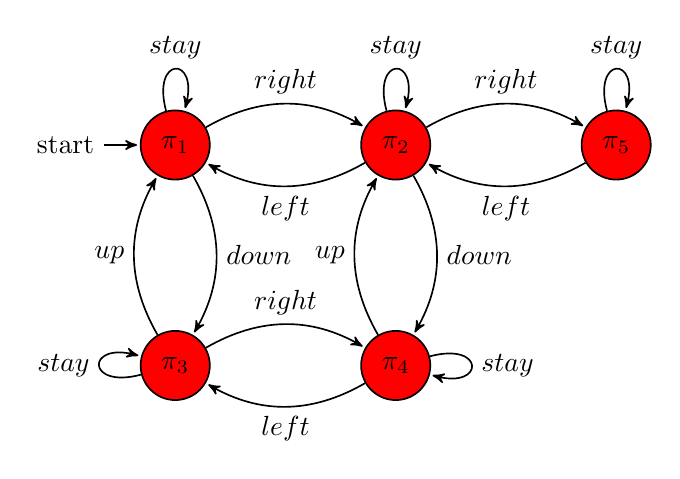
\begin{tikzpicture}[->,>=stealth',shorten >=1pt,auto,node distance=2.8cm,
                    semithick]
  \tikzstyle{every state}=[fill=red,draw=black,text=black]

  \node[initial,state] (A)                    {$\pi_1$};
  \node[state]         (B) [ right of=A] {$\pi_2$};
  \node[state]         (C) [below of=A] {$\pi_3$};
  \node[state]         (D) [right of=C] {$\pi_4$};
  \node[state]         (E) [right of=B] {$\pi_5$};

  \path (A) edge     [bend left]         node {$right$} (B)
  		(B) edge     [bend left]         node {$left$} (A)
		(A) edge     [bend left]         node {$down$} (C)
  		(C) edge     [bend left]         node {$up$} (A)
  		(C) edge     [bend left]         node {$right$} (D)
  		(D) edge     [bend left]         node {$left$} (C)
  		(B) edge     [bend left]         node {$down$} (D)
  		(D) edge     [bend left]         node {$up$} (B)
  		(B) edge     [bend left]         node {$right$} (E)
  		(E) edge     [bend left]         node {$left$} (B)
        (A) edge [loop above] node {$stay$} (A)
        (B) edge [loop above] node {$stay$} (B)
        (C) edge [loop left] node {$stay$} (C)
        (D) edge [loop right] node {$stay$} (D)
        (E) edge [loop above] node {$stay$} (E);
\end{tikzpicture}
\caption{Simple Finite Transition System}
\label{fig:ftsEx}
\end{figure}
This FTS will be used in figures unless otherwise stated. We chose it to be very simple because the state explosion problem applies even to this report. If we chose a more complex FTS we would not be able to include illustrations of the product automaton because it gets very big very quickly. We will henceforth refer to this FTS as simple FTS. When providing computational results, we will use an FTS that is much larger, to bring out the difference between our algorithm and the accepted algorithm.


\subsection{Reachability while avoiding regions} 
Reachability while avoiding regions is a property in which we wish to not cross over certain areas, say $\pi_1, \pi_2, \dots, \pi_n$, until we get to a specified region, say $\pi_{n+1}$. After reaching $\pi_{n+1}$ we are free to do what we want. This behaviour is expressed by the formula $\neg (\pi_1 \lor \pi_2 \lor \dots \pi_n) \U \pi_{n+1}$. 

The B\"{u}chi automaton corresponding to this formula is given in figure \ref{fig:ReachAvoid}

\begin{figure}
\centering
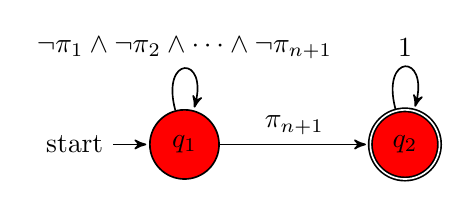
\begin{tikzpicture}[->,>=stealth',shorten >=1pt,auto,node distance=2.8cm,
                    semithick]
  \tikzstyle{every state}=[fill=red,draw=black,text=black]

  \node[initial,state] (A)                    {$q_1$};
  \node[state,accepting]         (B) [right of=A] {$q_2$};

  \path (A) edge              node {$\pi_{n+1}$} (B)
  		(A) edge [loop above] node {$\neg \pi_1 \wedge \neg \pi_2 \wedge \dots \wedge \neg \pi_{n+1}$} (A)
  		(B) edge [loop above] node {$1$} (B);
\end{tikzpicture}
\caption{B\"{u}chi automaton corresponding to $\neg (\pi_1 \lor \pi_2 \lor \dots \pi_n) \U \pi_{n+1}$}
\label{fig:ReachAvoid}
\end{figure}

As we can see $d_p(q_1)=1$ and $d_p(q_1)=0$. For our example, we will look at the specific formula $\neg \pi_4 \U \pi_5$ The product automaton is shown in figure \ref{fig:reachAvoidProduct}

\begin{figure*}
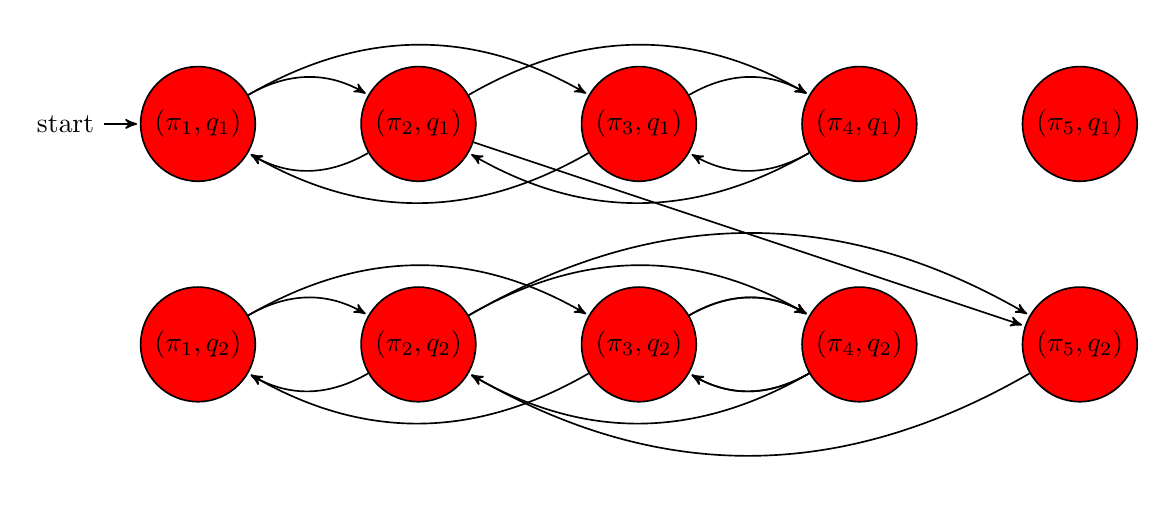
\begin{tikzpicture}[->,>=stealth',shorten >=1pt,auto,node distance=2.8cm,
                    semithick]
  \tikzstyle{every state}=[fill=red,draw=black,text=black]

  \node[initial,state] (A)                    {$(\pi_1,q_1)$};
  \node[state]         (B) [ right of=A] {$(\pi_2,q_1)$};
  \node[state]         (C) [right of=B] {$(\pi_3,q_1)$};
  \node[state]         (D) [right of=C] {$(\pi_4,q_1)$};
  \node[state]         (E) [right of=D] {$(\pi_5,q_1)$};
  
  \node[state] 		   (AA)  [below of=A]  {$(\pi_1,q_2)$};
  \node[state]         (BB) [ right of=AA] {$(\pi_2,q_2)$};
  \node[state]         (CC) [right of=BB] {$(\pi_3,q_2)$};
  \node[state]         (DD) [right of=CC] {$(\pi_4,q_2)$};
  \node[state]         (EE) [right of=DD] {$(\pi_5,q_2)$};  

  \path (A) edge     [bend left]          (B)
        (B) edge     [bend left]          (A)
        (A) edge     [bend left]         (C)
        (C) edge     [bend left]          (A)
        (C) edge     [bend left]          (D)
        (D) edge     [bend left]          (C)
		(B) edge     [bend left]          (D)
        (D) edge     [bend left]          (B)
        (B) edge               (EE)
        (DD) edge       [bend left]        (BB)
        (BB) edge        [bend left]       (DD)
        (BB) edge        [bend left]       (AA)
        (AA) edge        [bend left]       (BB)
        (BB) edge        [bend left]       (EE)
        (EE) edge        [bend left]       (BB)
        (DD) edge       [bend left]        (CC)
        (CC) edge        [bend left]       (DD)
        (CC) edge        [bend left]       (DD)
        (DD) edge        [bend left]       (CC)
        (CC) edge        [bend left]       (AA)
        (AA) edge        [bend left]       (CC);
\end{tikzpicture}
\caption{Product Automaton for $\neg \pi_4 \U \pi_5$ with Simple FTS}
\label{fig:reachAvoidProduct}
\end{figure*}
Note: in figure \ref{fig:reachAvoidProduct} all nodes have a self loop, which are not included for the sake of the reader.
Our algorithm does $n+1$ Dijkstra searches where $n$ is the maximum level of a state in the B\"{u}chi automaton. As we can see in \ref{fig:ReachAvoid}, which is the B\"{u}chi automaton corresponding to the general from of reachability while avoiding regions, $n$ is 1 for all formulas of this form. Therefore our algorithm does one Dijkstra search starting from $(\pi_1,q_1)$ which ends at $(\pi_5,q_2)$. This is exactly what the accepted algorithm does, so we do not gain anything when using our algorithm on a formula of this type.



\subsection{Sequencing}
Sequencing is the behaviour of visiting regions $\pi_1,\pi_2,\dots,\pi_n$ in that order. A formula that describes this behaviour for $n=3$ is $\diamond (\pi_1 \land \diamond(\pi_2 \land \diamond \pi_3))$ and is shown in figure \ref{fig:seq}. This behaviour is ideal for our algorithm.


\begin{figure}
\centering
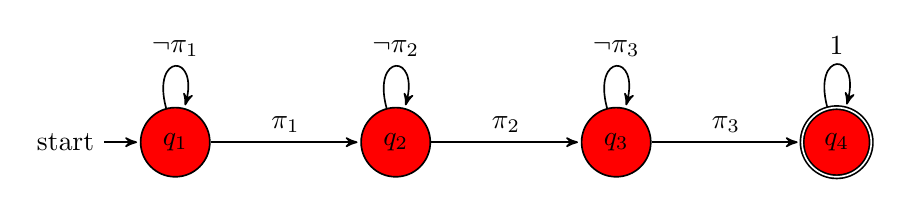
\begin{tikzpicture}[->,>=stealth',shorten >=1pt,auto,node distance=2.8cm,
                    semithick]
  \tikzstyle{every state}=[fill=red,draw=black,text=black]

  \node[initial,state] (A)                    {$q_1$};
  \node[state] (B)                    [right of=A]{$q_2$};
  \node[state] (C)                    [right of=B]{$q_3$};
  \node[state,accepting]         (D) [right of=C] {$q_4$};

  \path (A) edge              node {$\pi_{1}$} (B)
  		(A) edge [loop above] node {$\neg \pi_1$} (A)
  		(B) edge [loop above] node {$\neg \pi_2$} (B)
  		(B) edge              node {$\pi_{2}$} (C)
  		(C) edge [loop above] node {$\neg \pi_3$} (C)
  		(C) edge              node {$\pi_{3}$} (D)
  		(D) edge [loop above] node {$1$} (D);
\end{tikzpicture}
\caption{B\"uchi Automaton Corresponding to $\diamond (\pi_1 \land \diamond(\pi_2 \land \diamond \pi_3))$}
\label{fig:seq}
\end{figure}

We show why in an example using the formula $\diamond (\pi_2 \wedge \diamond \pi_5))$ the simple FTS as before. The product automaton is shown in figure \ref{fig:Sequencing}
\begin{figure*}
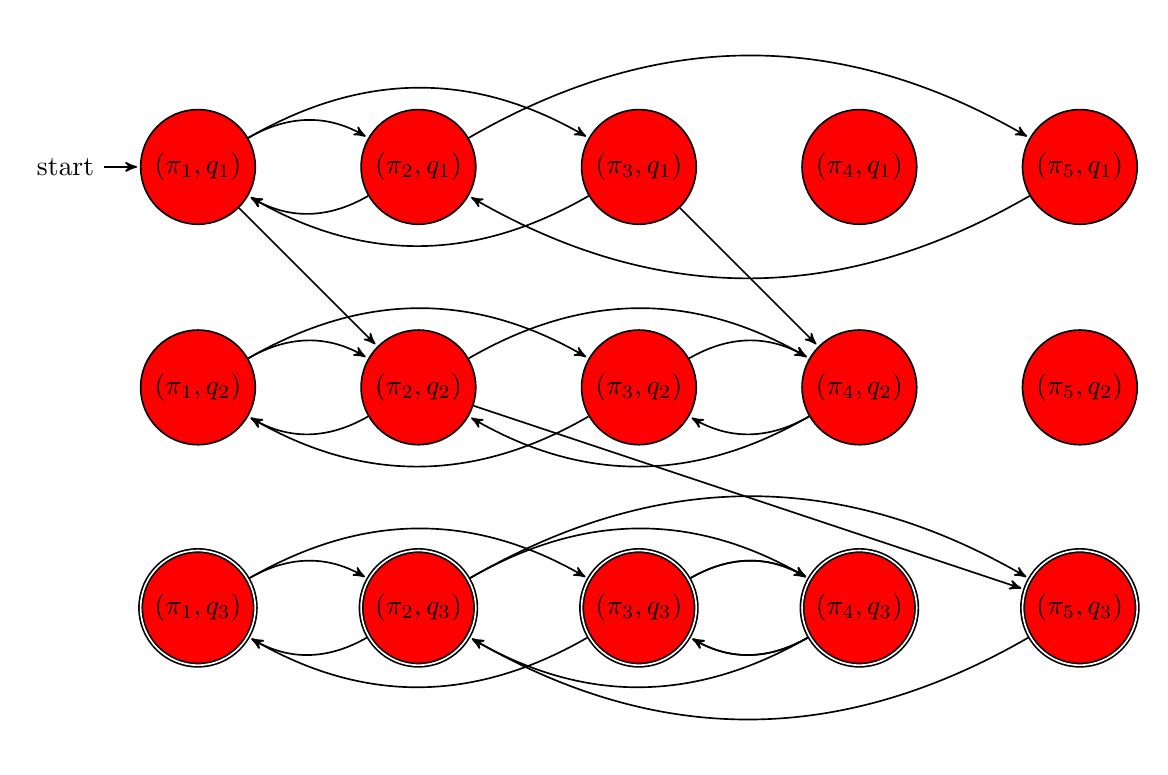
\begin{tikzpicture}[->,>=stealth',shorten >=1pt,auto,node distance=2.8cm,
                    semithick]
  \tikzstyle{every state}=[fill=red,draw=black,text=black]

  \node[initial,state] (A)                    {$(\pi_1,q_1)$};
  \node[state]         (B) [ right of=A] {$(\pi_2,q_1)$};
  \node[state]         (C) [right of=B] {$(\pi_3,q_1)$};
  \node[state]         (D) [right of=C] {$(\pi_4,q_1)$};
  \node[state]         (E) [right of=D] {$(\pi_5,q_1)$};
  
  \node[state] 		   (AA)  [below of=A]  {$(\pi_1,q_2)$};
  \node[state]         (BB) [ right of=AA] {$(\pi_2,q_2)$};
  \node[state]         (CC) [right of=BB] {$(\pi_3,q_2)$};
  \node[state]         (DD) [right of=CC] {$(\pi_4,q_2)$};
  \node[state]         (EE) [right of=DD] {$(\pi_5,q_2)$};
  
  \node[state,accepting] 		   (AAA)  [below of=AA]  {$(\pi_1,q_3)$};
  \node[state,accepting]         (BBB) [ right of=AAA] {$(\pi_2,q_3)$};
  \node[state,accepting]         (CCC) [right of=BBB] {$(\pi_3,q_3)$};
  \node[state,accepting]         (DDD) [right of=CCC] {$(\pi_4,q_3)$};
  \node[state,accepting]         (EEE) [right of=DDD] {$(\pi_5,q_3)$};
  

  \path (A) edge     [bend left]          (B)
        (B) edge     [bend left]          (A)
        (A) edge     [bend left]         (C)
        (C) edge     [bend left]          (A)
        (A) edge               (BB)
        (BB) edge               (EEE)
        (C) edge               (DD)
        (B) edge       [bend left]        (E)
        (E) edge       [bend left]        (B)
        %(B) edge       [bend left]        (D)
        %(D) edge       [bend left]        (B)
        (DD) edge       [bend left]        (BB)
        (BB) edge        [bend left]       (DD)
        (BB) edge        [bend left]       (AA)
        (AA) edge        [bend left]       (BB)
        (CC) edge        [bend left]       (AA)
        (AA) edge        [bend left]       (CC)
        (CC) edge        [bend left]       (DD)
        (DD) edge        [bend left]       (CC)
        
        (DDD) edge       [bend left]        (BBB)
        (BBB) edge        [bend left]       (DDD)
        (BBB) edge        [bend left]       (AAA)
        (AAA) edge        [bend left]       (BBB)
        (BBB) edge        [bend left]       (EEE)
        (EEE) edge        [bend left]       (BBB)
        (DDD) edge       [bend left]        (CCC)
        (CCC) edge        [bend left]       (DDD)
        (CCC) edge        [bend left]       (DDD)
        (DDD) edge        [bend left]       (CCC)
        (CCC) edge        [bend left]       (AAA)
        (AAA) edge        [bend left]       (CCC);
\end{tikzpicture}
\caption{Product Automaton for $\diamond (\pi_2 \wedge \diamond \pi_5))$ with Simple FTS}
\label{fig:Sequencing}
\end{figure*}

Our algorithm finds $(\pi_4,q_2)$, then starts another Dijkstra search and finds $(\pi_5,q_3)$. Will search through extraneous nodes, for example $(\pi_5,q_1)$. This may not seem like a lot in this example, but when we expand to larger problems the difference becomes significant. Check how many nodes are searched with both algorithms, and show time difference.

\subsection{Coverage}
A coverage formula represents the statement visit $\pi_1, \pi_2, \dots, \pi_n$ in that order, and is of the form $\varphi = \diamond \pi_1 \wedge \diamond \pi_2 \wedge \dots \wedge \pi_n$. We show the B\"uchi automaton corresponding to the formula $\diamond \pi_1 \wedge \diamond \pi_2 \wedge \pi_3$ in figure \ref{fig:buchCov}

\begin{figure}
\centering
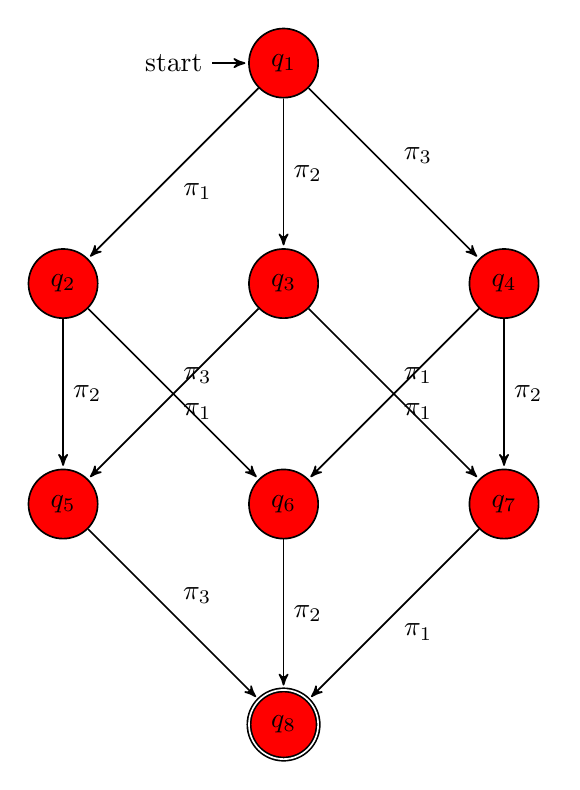
\begin{tikzpicture}[->,>=stealth',shorten >=1pt,auto,node distance=2.8cm,
                    semithick]
  \tikzstyle{every state}=[fill=red,draw=black,text=black]

  \node[initial,state] (A)                    {$q_1$};
  \node[state] (C)                    [below of=A]{$q_3$};
  \node[state] (D)                    [right of=C]{$q_4$};
  \node[state]         (B) [left of=C] {$q_2$};
  \node[state] (E) 					[below of=B]{$q_5$};
   \node[state] (F) 					[below of=C]{$q_6$};
   \node[state] (G) 					[below of=D]{$q_7$};
   \node[accepting,state] (H) 					[below of=F]{$q_8$};
  

  \path (A) edge              node {$\pi_{1}$} (B)
   (A) edge              node {$\pi_{2}$} (C)
   (A) edge              node {$\pi_{3}$} (D)
   (B) edge              node {$\pi_{2}$} (E)
   (B) edge              node {$\pi_{3}$} (F)
   (C) edge              node {$\pi_{1}$} (E)
   (E) edge              node {$\pi_{3}$} (H)
   (F) edge              node {$\pi_{2}$} (H)
   (G) edge              node {$\pi_{1}$} (H)
   (D) edge              node {$\pi_{2}$} (G)
   (D) edge              node {$\pi_{1}$} (F)
   (C) edge              node {$\pi_{1}$} (G);
\end{tikzpicture}
\caption{B\"uchi Automaton Corresponding to $\diamond \pi_1 \wedge \diamond \pi_2 \wedge \pi_3$}
\label{fig:buchCov}
\end{figure}

So, we can see that to get to the accepting node, we have to choose which node to go to first, and which node to go to second (the third node we then have to visit is already decided). So, there are 6 possible paths to take from the initial node, $q_1$ to accepting state $q_8$. This is true in the product automaton too, if we only consider the option of taking the optimal path between nodes. The order that our algorithm will pick is it will pick first pick $\pi_i$ which is the closest to it. From then, it will pick the next closest $\pi_j$ out of the two that have not been visited yet.

We now define a workspace to use with our problem. Our workspace is a grid, 25 units across and 25 units up, a total of 625 regions. We say our robot can can move horizontally and vertically, however it cannot move diagonally. Additionally we say that the unit cost of going from any adjacent to another region is 1. The initial position is located at $(0,0)$, region $\pi_1$ is located at (2,24), region $\pi_2$ is located at (12,12), and region $\pi_3$ is located at (20,15) . See figure \ref{fig:workspace}

\begin{figure}[!htb]
\centering
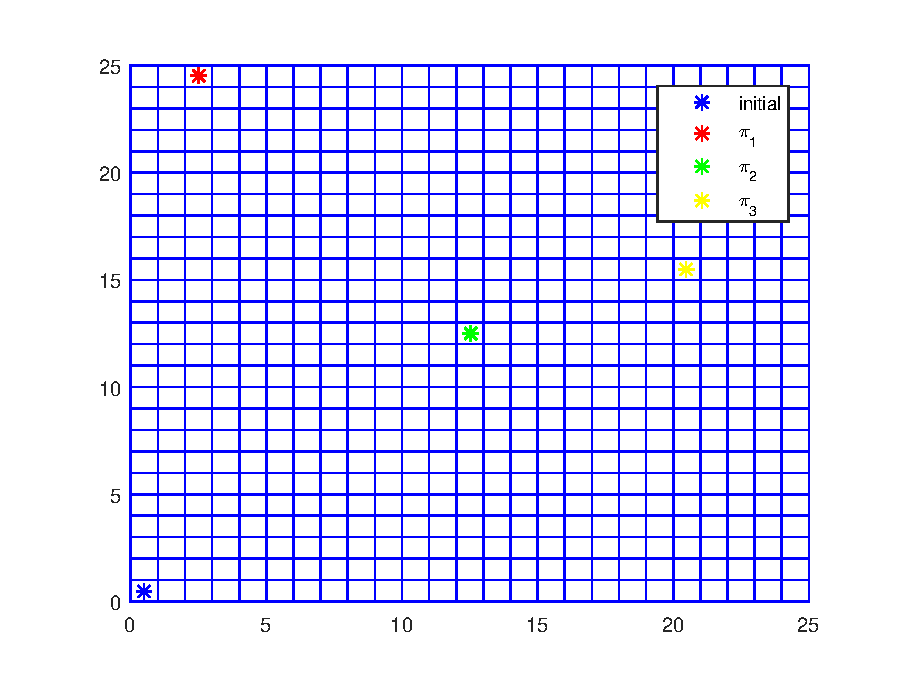
\includegraphics[scale=1]{workspace.eps}
\label{fig:workspace}
\end{figure}


When we use our algorithm on a coverage formula, we may not get the optimal path. We will however get an accepting path, and we now show that this path corresponds to the one generated by the nearest neighbour approach to the travelling salesperson problem. We also provide a provide a bound on the distance of our path based on the worst case ratio of the nearest neighbour tour to the optimal tour given by Rosendrantz, Stearns, and Lewis \cite{rosenkrantz74}. The travelling salesperson problem is stated in layman's terms as finding the shortest path for a salesperson to take such that he passes through a given set of cities and then returns back home at the end. More formally, it can be stated as finding the minimum Hamiltonian circuit with the lowest sum of distances between the nodes (cities). This problem has been studied extensively and "give quote about importance". This problem is NP-hard, and thus many algorithms and heuristics exist for finding an approximate solution. One very simple algorithm to do this is called the nearest neighbour algorithm. It says from the starting city, pick the closest city to be the next stop. From there, pick the next closest city not including the starting city, and so on. If there is a tie in the next closest neighbour, we assume that the next node can be decided arbitrarily. This is exactly what our algorithm does in this situation, the first Dijkstra search finds the closest node, and the we start another search. 

To formulate our problem as a travelling salesman problem we use the idea of a dummy node from Lenstra and Rinnooy Kan's computer wiring example in \cite{lenstra75}. In their example, they are designing a computer interface at the Institute for Nuclear Physical Research in Amsterdam. An interface is made up of several modules, with multiple pins on each module. A given subset of pins has to be interconnnected by wires, and at most two wires can be connected to any pin. For obvious regions, it is desirable to minimize the amount of wire used. They show that this is actually a travelling salesperson problem in disguise. The only difference between this problem and a travelling salesman problem is that in the travelling salesman problem, the salesman must return home at the end. This is not true in this problem. It is also not true in our problem, we only need to pass through $\pi_1$, $\pi_2$ and $\pi_3$, there is no need to return to the starting state after we do this. To formulate this seemingly unrelated problem into a travelling salesperson problem, they set $P$ to be the set of pins to be interconnected, $c_{ij}$ to be the distance between pin $i$ and pin $j$. They then introduce a dummy node $*$ that is a distance 0 from all the other nodes i.e.\ $c_{i*} = c_{*i} = 0$ for all i. Then the corresponding problem is solving the travelling salesperson problem on the set of nodes $N=P \cup \{*\}$. 

For our problem, we set $c_{ij}=d(\pi_i , \pi_j)$, for $i,j=0,1,2,3$ where where the initial state is from now on known as $\pi_0$, to be the shortest path our robot can take from $\pi_i$ to $\pi_j$, insuring that the triangle inequality is satisfied for all $i$ and $j$. We must preserve the the triangle inequality for a proof of a worst case scenario bound we will provide later on. We use this same idea as above of adding a dummy node, however to preserve the triangle inequality we cannot have the dummy node be distance 0 from the other nodes. Indeed, if $c_{i*} = c_{*i} = 0 $ the triangle inequality would be violated because $c_{i*} + c_{*j} = 0 \geq c_{ij}$ which would make the cost from getting to any point 0, thus rendering the problem extremely trivial. 

We can represent the relationship between the regions in our graph with the following \textit{complete} subgraph, shown in figure. A complete graph is an undirected graph in which every pair of vertices is connected by an edge. 
\begin{figure}
\centering
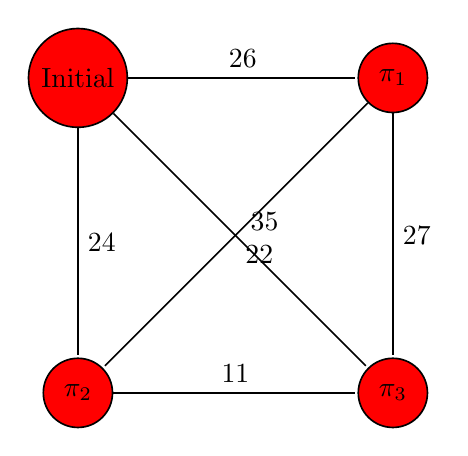
\begin{tikzpicture}[-,>=stealth',shorten >=1pt,auto,node distance=4cm,
                    semithick]
  \tikzstyle{every state}=[fill=red,draw=black,text=black]

  \node[state] (A)                    {Initial};
  \node[state] (B)                    [right of=A]{$\pi_1$};
  \node[state] (C)                    [below of=A]{$\pi_2$};
  \node[state]         (D) [right of=C] {$\pi_3$};

  \path (A) edge              node {$26$} (B)
  		(A) edge 			 node {$24$} (C)
  		(A) edge              node {$35$} (D)
  		(B) edge 				node {$22$} (C)
  		(B) edge              node {$27$} (D)
  		(C) edge				node {$11$} (D);
\end{tikzpicture}
\caption{Complete Graph between Regions of Interest}
\label{fig:completeGraph}
\end{figure}

For the distances, we use the so called \textit{Manhattan distance}, i.e.\ $d((x_1,y_1),(x_2,y_2)) = |x_1 - x_2| +| y_1 - y_2|$ because our robot can only move horizontally and vertically, not diagonally. Given the weights between the vertices, we easily see that the path that our algorithm, and the nearest neighbour, will take is shown in figure \ref{fig:pathOnComplete}. The cost of this path is 62.

\begin{figure}
\centering
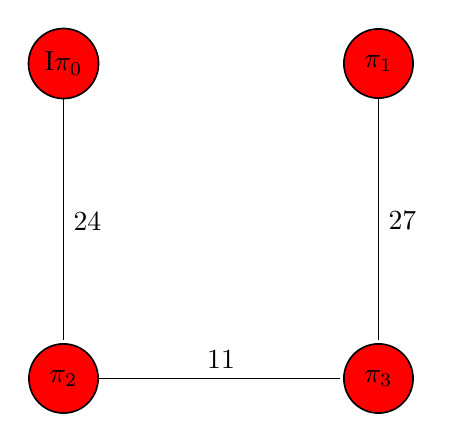
\begin{tikzpicture}[-,>=stealth',shorten >=1pt,auto,node distance=4cm,
                    semithick]
  \tikzstyle{every state}=[fill=red,draw=black,text=black]

  \node[state] (A)                    {I$\pi_0$};
  \node[state] (B)                    [right of=A]{$\pi_1$};
  \node[state] (C)                    [below of=A]{$\pi_2$};
  \node[state]         (D) [right of=C] {$\pi_3$};

  \path (A) edge 			 node {$24$} (C)
  		(B) edge              node {$27$} (D)
  		(C) edge				node {$11$} (D);
\end{tikzpicture}
\caption{Nearest Neighbour Path}
\label{fig:pathOnComplete}
\end{figure}

This is not the optimal path though, which is shown in figure \ref{fig:optcompleteGraph} and has a cost of 59.

\begin{figure}
\centering
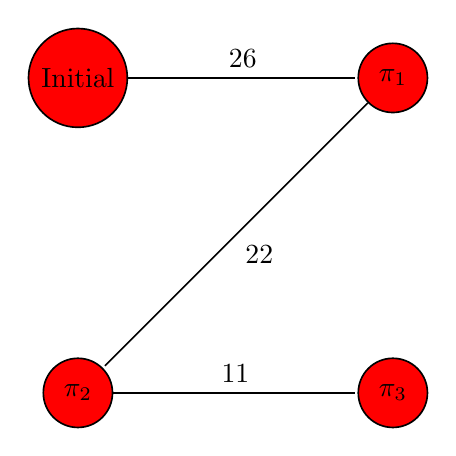
\begin{tikzpicture}[-,>=stealth',shorten >=1pt,auto,node distance=4cm,
                    semithick]
  \tikzstyle{every state}=[fill=red,draw=black,text=black]

  \node[state] (A)                    {Initial};
  \node[state] (B)                    [right of=A]{$\pi_1$};
  \node[state] (C)                    [below of=A]{$\pi_2$};
  \node[state]         (D) [right of=C] {$\pi_3$};

  \path (A) edge              node {$26$} (B)
  		%(A) edge 			 node {$24$} (C)
  		%(A) edge              node {$35$} (D)
  		(B) edge 				node {$22$} (C)
  		%(B) edge              node {$27$} (D)
  		(C) edge				node {$11$} (D);
\end{tikzpicture}
\caption{Optimal Path}
\label{fig:optcompleteGraph}
\end{figure}


Because we have to make sure that the dummy node does not change the order that our algorithm and the nearest neighbour algorithm takes we have to set the distance the dummy node is away from every other node to be $max_{i,j} c_{ij} $ where $c_{ij}$ is the distance between the nodes in the complete subgraph in figure \ref{fig:completeGraph}. In our case, this is 35, the path between $\pi_0$ and $\pi_3$. This insures that the path taken is the same as the accepted neighbour because the dummy node will be the last node to be visited. This is because in the nearest neighbour algorithm, ties are broken arbitrarily. Thus, the only time where it is a possibility that the nearest neighbour algorithm goes to the dummy node i.e.\ when the next nodes are $\max_{i,j} c_{ij}$ from the current node is when and if we are faced with the only choice being take the maximum path $\max_{i,j} c_{i,j}$ to $\pi_j$ or to go to the dummy node, and we can choose to go to $\pi_j$ because the ties can be broken arbitrarily. In any other case, the nearest neighbour path will choose a to go to a node where the cost is $c_{i',j'} < c_{i,j}$. 

We show the new subgraph in figure \ref{fig:completeDummy}

\begin{figure}
\centering
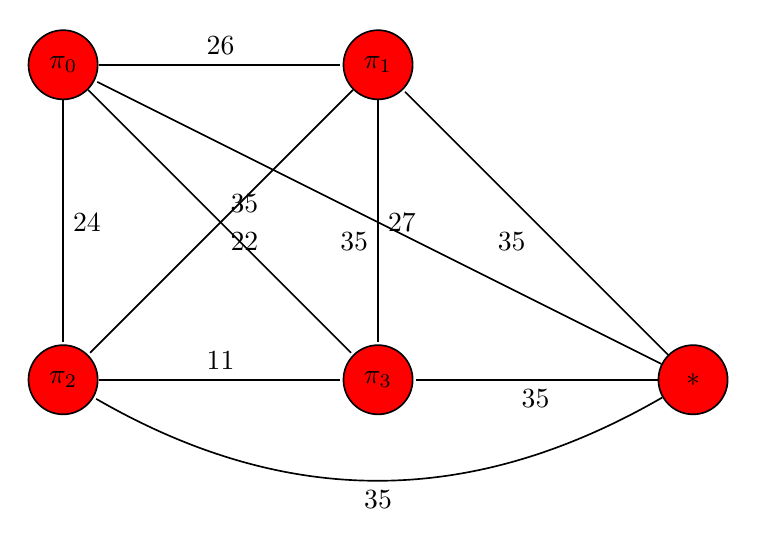
\begin{tikzpicture}[-,>=stealth',shorten >=1pt,auto,node distance=4cm,
                    semithick]
  \tikzstyle{every state}=[fill=red,draw=black,text=black]

  \node[state] (A)                    {$\pi_0$};
  \node[state] (B)                    [right of=A]{$\pi_1$};
  \node[state] (C)                    [below of=A]{$\pi_2$};
  \node[state]         (D) [right of=C] {$\pi_3$};
  \node[state] (E)			[right of = D] {$*$}; 

  \path (A) edge              node {$26$} (B)
  		(A) edge 			 node {$24$} (C)
  		(A) edge              node {$35$} (D)
  		(B) edge 				node {$22$} (C)
  		(B) edge              node {$27$} (D)
  		(C) edge				node {$11$} (D)
  		(E) edge 				node {$35$} (D)
  		(E) edge 				[bend left] node {$35$} (C)
  		(E) edge 				node {$35$} (B)
  		(E) edge 				node {$35$} (A);
\end{tikzpicture}
\caption{Complete Subgraph with Dummy Node}
\label{fig:completeDummy}
\end{figure}

The path that the nearest neighbour algorithm takes in this situation, the complete Hamiltonian circuit, is given in figure \ref{fig:NearNeigDummy}, which gives a total cost of 132.

\begin{figure}
\centering
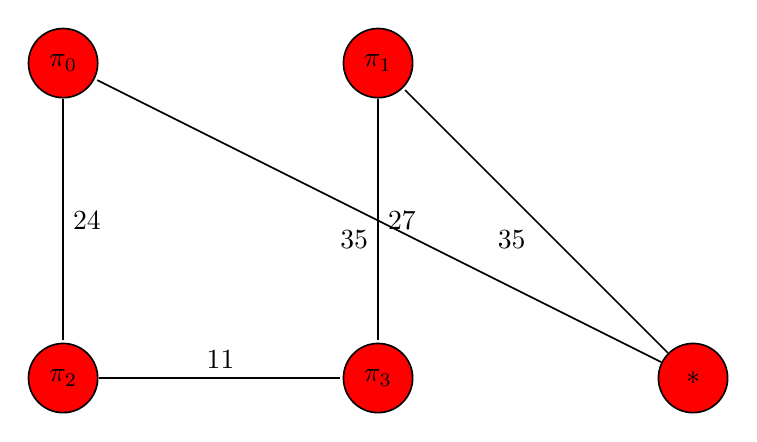
\begin{tikzpicture}[-,>=stealth',shorten >=1pt,auto,node distance=4cm,
                    semithick]
  \tikzstyle{every state}=[fill=red,draw=black,text=black]

  \node[state] (A)                    {$\pi_0$};
  \node[state] (B)                    [right of=A]{$\pi_1$};
  \node[state] (C)                    [below of=A]{$\pi_2$};
  \node[state]         (D) [right of=C] {$\pi_3$};
  \node[state] (E)			[right of = D] {$*$}; 

  \path (A) edge 			 node {$24$} (C)
  		%(A) edge              node {$35$} (D)
  		%(B) edge 				node {$22$} (C)
  		(B) edge              node {$27$} (D)
  		(C) edge				node {$11$} (D)
  		%(E) edge 				node {$35$} (D)
  		%(E) edge 				[bend left] node {$35$} (C)
  		(E) edge 				node {$35$} (B)
  		(E) edge 				node {$35$} (A);
\end{tikzpicture}
\caption{Nearest Neighbour Path with Dummy Node}
\label{fig:NearNeigDummy}
\end{figure}

We node however that this is not the optimal solution. This optimal solution is shown in 
figure \ref{fig:optDummy} and has a cost of 129.

\begin{figure}
\centering
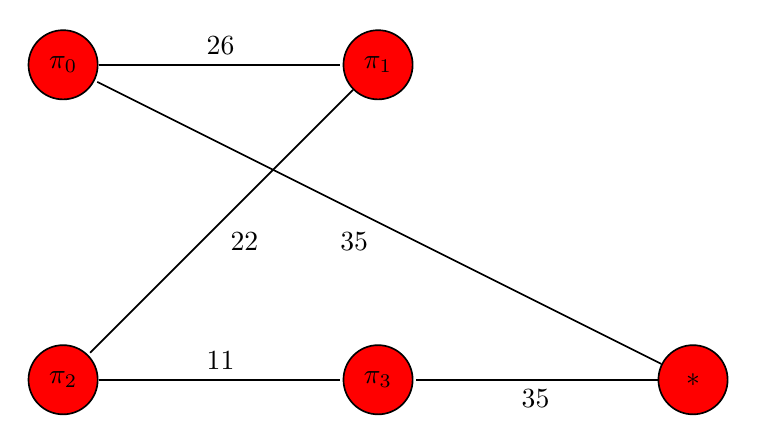
\begin{tikzpicture}[-,>=stealth',shorten >=1pt,auto,node distance=4cm,
                    semithick]
  \tikzstyle{every state}=[fill=red,draw=black,text=black]

  \node[state] (A)                    {$\pi_0$};
  \node[state] (B)                    [right of=A]{$\pi_1$};
  \node[state] (C)                    [below of=A]{$\pi_2$};
  \node[state]         (D) [right of=C] {$\pi_3$};
  \node[state] (E)			[right of = D] {$*$}; 

  \path (A) edge			node {$26$} (B)
  		%(A) edge 			 node {$24$} (C)
  		%(A) edge              node {$35$} (D)
  		(B) edge 				node {$22$} (C)
  		%(B) edge              node {$27$} (D)
  		(C) edge				node {$11$} (D)
  		(E) edge 				node {$35$} (D)
  		%(E) edge 				[bend left] node {$35$} (C)
  		%(E) edge 				node {$35$} (B)
  		(E) edge 				node {$35$} (A);
\end{tikzpicture}
\caption{Optimal Path with Dummy Node}
\label{fig:optDummy}
\end{figure}



It has been shown that for an n-node travelling salesperson problem which satisfies the triangle inequality i.e.\ $d(i,j) = d(j,k) \geq d(i,k)$ for all $i,j,$ and $k$ where $d(i,j)$ is the nonnegative distance between nodes $i$ and $j$, 
\begin{align*}
\text{NEARNEIBR} \leq (\frac{1}{2} \lceil \log(n) \rceil + \frac{1}{2})\text{OPTIMAL}
\end{align*}
where NEARNEIBR is the cost of the path generated by the nearest neighbour algorithm and OPTIMAL is the cost of the optimal path. 

Our values do indeed satisfy this inequality
\begin{align*}
\text{NEARNEIBR} &\leq (\frac{1}{2} \lceil \log(n) \rceil + \frac{1}{2})\text{OPTIMAL} \\
132 &\leq (\frac{1}{2} \lceil \log(5) \rceil + \frac{1}{2})129 \\
132 &\leq (2)129 \\
132 \leq 258 
\end{align*}
We also see that it is very conservative worst case bound and we will likely do much better.

We provide a proof of
\begin{align}
\dfrac{\text{NEARNEIBR}}{\text{OPTIMAL}} \leq \frac{1}{2} \lceil \log(n) \rceil + \frac{1}{2}
\end{align}
which can be found in \cite{rosenkrantz74}. 
Proof:
We begin by proving 
\begin{align}
\text{OPTIMAL} \geq 2 \sum^{\min(2k,n)}_{i=k+1} l_i \label{eq:showFirst}
\end{align}
for all $k$, $0\leq k \leq n$. 
Let $l_i$ be the length of the $i^{th}$ largest edge in the tour obtained by the nearest neighbour algorithm. For each $i$, $0 \leq i \leq n$, let $a_i$ be the node \textit{onto which} the $i^{th}$ largest edge is added to (that would be the edge with length $l_i$). Let $H$ be the complete subgraph defined on the set of nodes $\{a_i | 1 \leq i \leq min(2k,n)\}$.

Now, let $T$ be the tour in $H$ which visits the nodes of $H$ in the same order as these nodes are visited in an optimal tour of the original graph. Let LENGTH be the length of $T$. We have 
\begin{align}
\text{OPTIMAL $\geq$ LENGTH} \label{eq:optglen}
\end{align}
This is because the tour with cost OPTIMAL passes through all the nodes that the tour with cost LENGTH passes through, and more. Thus if H has an edge $(b,c)$, then the OPTIMAL tour will either have the edge $(b,c)$ or take a less direct route through some of its extra nodes. So the triangle inequality implies (\ref{eq:optglen}).  
   
Let $(a_i,a_j)$ be an edge of $T$. If the nearest neighbour method adds point $a_i$ before $a_j$, we have $d(a_i,a_j) \geq l_i$, where $d(a_i,a_j)$ is the distance between nodes $a_i$ and $a_j$. We also see that if $a_j$ is added first we have $d(a_i, a_j) \geq l_j$. This is because, say we added $a_i$ first, we know there is a point $l_i$ away from $a_i$ that the nearest neighbour method makes the path to. This can be $a_j$, because we know $a_j$ has not been added yet or another node. If it is another node $d(a_i, a_j) \geq l_i$ because the nearest neighbour finds the closest node that has not yet been visited, or $d(a_i, a_j) = l_i$ if $a_j$ is added next. 

Since one has to be added before the other, we have 
\begin{align}
d(a_i , a_j) \geq \min(l_i, l_j) \label{ex:oneBefore}
\end{align}

Summing (\ref{ex:oneBefore}) over the edges of $T$, we get
\begin{align}
\text{LENGTH} \geq \sum_{(a_i,a_j) \text{ in } T} \min(l_i,l_j)  \label{eq:lengmin}
\end{align}

If we let $\alpha_i$ be the number of edges $(a_i, a_j)$ in $T$ for which $l_i$ is selected as $\min(l_i, l_j)$ we obtain 

\begin{align}
\sum_{(a_i,a_j) \text{ in } T} \min(l_i, l_j) = \sum_{a_i \text{ in } H} a_i l_i  \label{ex:lowBound}
\end{align}

Because $a_i$ is the endpoint of two edges in $T$, $\alpha \leq 2$. 

Because $T$ has $\min(2k,n)$ edges (one for each node),

\begin{align}
\sum_{a_i \text{ in } H} \alpha_i = \min(2k,n) 
\end{align}

To get a lower bound on (\ref{ex:lowBound}) we assume that $\alpha_i = 2 $ for $k+1 \leq i \leq \min(2k,n)$ and is zero of $i \leq k$. Thus,

\begin{align}
\sum_{a_i \text{ in } H} a_i l_i \geq 2 \sum_{i=k+1}^{\min(2k,n)} l_i \label{eq:alg2}
\end{align}

Combining (\ref{eq:optglen}), (\ref{eq:lengmin}), (\ref{ex:lowBound}), and (\ref{eq:alg2}), we get

\begin{align*}
\text{OPTIMAL} \geq \text{LENGTH} \geq \sum_{(a_i,a_j) \text{ in } T} \min(l_i,l_j) = \sum_{a_i \text{ in } H} a_i l_i \geq 2 \sum_{i=k+1}^{\min(2k,n)} l_i
\end{align*}
thus proving (\ref{eq:showFirst}). 

We now sum (\ref{eq:showFirst}) for all values of $k$ for all values of $k$ equal to powers of two less than or equal to $n$ i.e. $k = 2^{j} \leq n$ for $j = 0, 1, \dots \lceil \log(n) \rceil - 1$. We then get

\begin{align*}
\sum_{j=0}^{\lceil \log(n) \rceil -1} \text{OPTIMAL} \geq \sum_{j=0}^{\lceil \log(n) \rceil - 1} ( 2 \cdot \sum_{i=2^j + 1}^{\min(2^{j+1,n})} l_i )
\end{align*}
We have
\begin{align*}
\sum_{j=0}^{\lceil \log(n) \rceil -1} \text{OPTIMAL} &\geq 2 \cdot \sum_{i=2}^2 l_i + 2 \cdot \sum_{i=3}^4 l_i + 2 \cdot \sum_{i=5}^8 + \sum_{j=3}^{\lceil log(n) \rceil - 1} (2 \cdot \sum_{i = 2^j+1}^{\min(2^{j+1},n)} l_i )\\
& \geq 2 l_2 + 2 l_3 + 2 l_4 \dots +2l_8 + \sum_{j=3}^{\lceil log(n) \rceil - 1} (2 \cdot \sum_{i = 2^j+1}^{\min(2^{j+1},n)} l_i)
\end{align*}

Therefore we can write

\begin{align}
\lceil \log(n) \rceil \cdot \text{OPTIMAL} \geq 2 \sum_{i = 2}^n l_i \label{eq:lognoptt}
\end{align}

Now OPTIMAL must be longer than twice any edge in the graph because it contains two paths between any given pair of points and these paths are , by the triangle  inequality, longer than the distance of the edge connecting the points directly, i.e.\ OPTIMAL $\geq 2 l_i$ for $i = 1,2,\dots, n$. Specifically,
\begin{align}
\text{OPTIMAL} \geq 2 \l_1 \label{eq:optgl1}
\end{align}

Summing (\ref{eq:lognoptt}) and (\ref{eq:optgl1}) we get 
\begin{align*}
(\log(n)+1) \cdot \text{OPTIMAL} \geq 2 \sum_{i=1}^n l_i
\end{align*}
By definition, $\sum_{i=1}^n l_i = \text{NEARNEIBR}$, thus we have 
\begin{align*}
\text{NEARNEIBR} \leq (\frac{1}{2} \lceil \log(n) \rceil + \frac{1}{2}) \text{OPTIMAL}
\end{align*}
\qed 

We have thus shown that when formulating and solving our problem as a travelling salesman problem with a dummy node, we get the same solution as the nearest neighbour search algorithm. This search algorithm then has a bound on the ratio of the resulting path to the optimal path i.e.\ 
\begin{align*}
\frac{\text{NEARNEIBR}}{\text{OPTIMAL}} \leq (\frac{1}{2} \lceil \log(n) \rceil + \frac{1}{2}) 
\end{align*}

We now must remove the dummy node and provide a bound for the true cost that we will get from our search. 

NEARNEIBR and OPTIMAL as above are costs of Hamaltonian circuits. By definition every node in a Hamaltonian circuit is passed through exactly once. Therefore the dummy node will be passed through exactly once, and we have shown that it will be the last node passed through in the NEARNEIBR. In the NEARNEIBR path, because the dummy node is length $\max_{i,j} c_{i,j}$ it will never be the closest next node, unless we are given the choice to go from $\pi_i$ to $\pi_j$ for $i$ and $j$ being the maximum edge cost in the complete subgraph. In this case we can break the tie arbitrarily and choose to go to $\pi_j$ instead of the dummy node. Thus the path found by the nearest neighbour search will be the path found by our our algorithm, and then going to the dummy node for a cost of $\max_{i,j} c_{i,j}$, then from there going to the initial node to for a cost of $\max_{i,j} c_{i,j}$. Therefore the cost of our algorithm, denote ALGOR is 
\begin{align*}
\text{ALGOR = NEARNEIBR - } 2\max_{i,j} c_{i,j} 
\end{align*}

The path OPTIMAL, however is not guaranteed to have the dummy node be the last node visited. The cost of the path which is optimal and requires that the dummy node is the last node visited, is then greater than or equal to OPTIMAL. This is because of the freedom taken away by requiring the dummy node to be visited last, and less freedom in a minimization problem results in a larger value. Let ACCEPT be the cost of the accepted algorithm for path planning. ACCEPT $+ 2\max_{i,j} c_{i,j}$ is then equal to the cost of the optimal travelling salesman solution which requires that the dummy node is the last node visited. This is because we have already established that the accepted algorithm will find the optimal path. Therefore we have
\begin{align*}
\text{ACCEPT} + 2\max_{i,j} c_{i,j} \geq \text{OPTIMAL}
\end{align*}

Plugging into the travelling salesman bound, we get
\begin{align*}
\text{NEARNEIBR} &\leq (\frac{1}{2} \lceil \log(n) \rceil + \frac{1}{2}) \text{OPTIMAL} \\
\text{ALG} + 2\max_{i,j} c_{i,j} &\leq (\frac{1}{2} \lceil \log(n) \rceil + \frac{1}{2}) \text{OPTIMAL} \\
\text{ALG} + 2\max_{i,j} c_{i,j} &\leq (\frac{1}{2} \lceil \log(n) \rceil + \frac{1}{2}) (\text{ACCEPT} + 2 \max_{i,j} c_{i,j}) \\ 
\end{align*} 
%We can see $\frac{1}{2} \lceil \log(n) \rceil + \frac{1}{2} \geq 0$ for all $n \geq 1$. $n$ is the number of nodes so we can see that it is the case $n\geq 1$. We can  


We can check with our previously calculated values for ALG and ACCEPT
\begin{align*}
\text{ALG} + 2\max_{i,j} c_{i,j} &\leq (\frac{1}{2} \lceil \log(n) \rceil + \frac{1}{2}) (\text{ACCEPT} + 2 \max_{i,j} c_{i,j} \\ 
62 + 2 (35) &\leq (\frac{1}{2} 3 + \frac{1}{2})(59+2(35)) \\
132 &\leq 258
\end{align*}
We can see that this is still a conservative bound, and emphasize that it is the worst case. Usually the algorithm will preform much better.


\subsection{Recurrence (Liveness)}
Recurrence is coverage over and over again, and can be expressed as $\square(\diamond \pi_1 \land \diamond \pi_2 \land \dots \land \diamond \pi_n)$. This example is interesting for two reasons: it is prone to B\"{u}chi automata that are not tight, and it an accepting path for it does cannot stay in one state (in contrast to the other formulas, in which all accepting states have self loops). We first look at the tightness.

To illustrate our point, we consider the formula $\square(\diamond \pi_1 \land \diamond \pi_2 \land \diamond \pi_3)$. The B\"{u}chi automaton corresponding to this formula, as calculated by \cite{gastin01} is 

\begin{figure}
\centering
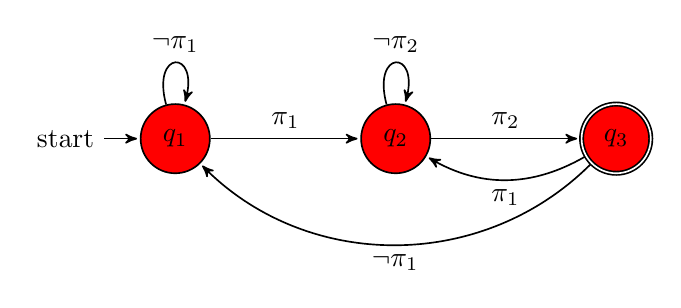
\begin{tikzpicture}[->,>=stealth',shorten >=1pt,auto,node distance=2.8cm,
                    semithick]
  \tikzstyle{every state}=[fill=red,draw=black,text=black]

  \node[initial,state] (A)                    {$q_1$};
  \node[state] (B)                    [right of=A]{$q_2$};
  \node[state,accepting] (C)                    [right of=B]{$q_3$};

  \path (A) edge              node {$\pi_{1}$} (B)
  		(A) edge [loop above] node {$\neg \pi_1$} (A)
  		(B) edge [loop above] node {$\neg \pi_2$} (B)
  		(B) edge              node {$\pi_{2}$} (C)
  		(C) edge [bend left=45] node {$\neg \pi_1$} (A)
  		(C) edge  [bend left] node {$\pi_{1}$} (B);
%  		(D) edge [bend right] node {$\neg \pi_1$} (A)
 % 		(D) edge [bend left] node {$\pi_1$} (B);
\end{tikzpicture}
\caption{B\"uchi Automaton for $\square(\diamond \pi_1 \land \diamond \pi_2 \land \diamond \pi_3)$ 1}
\label{fig:gasBuchiRec}
\end{figure}
Note: The actual automaton generated has much more edges. For example, there is an edge from $q_4$ to $q_2$ which is labelled $\pi_1 \&\& \pi_2$. It is impossible for us to make this transition because $\pi_i$ for all $i$ is a region in our partition. This is because the requirements of our partition are chosen specially to guarantee that we are never in two regions at once. Thus they are excluded in the interest of the reader. In this automation, $d(q_1)=2$, $d(q_2)=1$, and $d(q_3)=0$. So, to get from $q_{init}' = \langle \pi_2, q_1 \rangle \in Q_0'$, we have to first get down to level 2. Given the B\"{u}chi automaton \ref{fig:gasBuchiRec} the only way to do this is to go to region $\pi_1$. Our algorithm does this, and then starts a new Dijkstra search. In this case the same statement holds for $\pi_2$. Therefore the optimal prefix is to concatenate the optimal paths down from each each level (first to $\pi_1$, etc). Our algorithm does a Dijkstra search at each level so it will return this path as the prefix. The accepted algorithm will also return this prefix. 

This path however is in general not truly optimal. It is because the B\"{u}chi automaton given in figure \ref{fig:gasBuchiRec} not a tight B\"{u}chi automaton \cite{schuppan05}. A B\"{u}chi automaton is tight if it accepts the shortest lasso (prefix and suffix). The loss of this optimality property is due to the fact that the algorithm in \cite{gastin01} simplifies the B\"{u}chi automaton which is usually a good thing because it leads to a lower computational complexity in most applications. We take a look at a different automaton corresponding to the formula $\square(\diamond \pi_1 \land \diamond \pi_2)$, shown in figure \ref{fig:otherBuchiRec}. 

\begin{figure*}
\centering
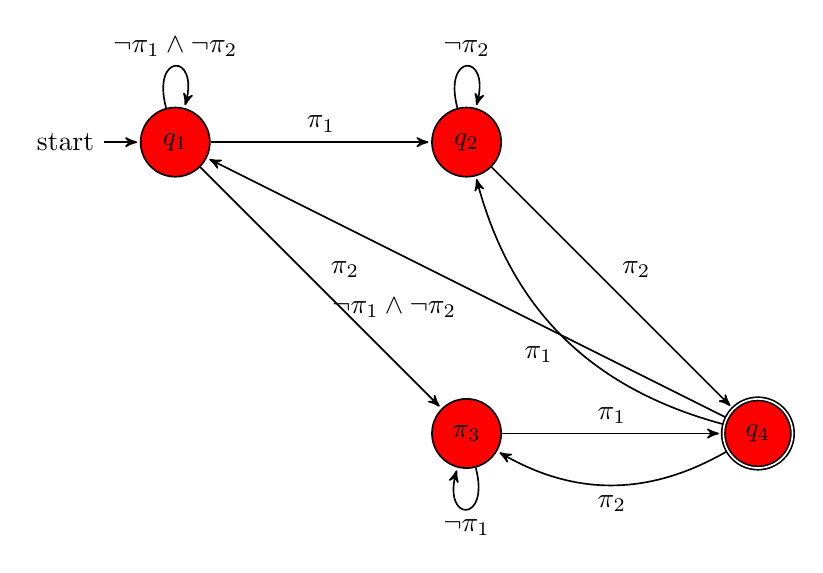
\begin{tikzpicture}[->,>=stealth',shorten >=1pt,auto,node distance=3.7cm,
                    semithick]
  \tikzstyle{every state}=[fill=red,draw=black,text=black]

  \node[initial,state] (A)                    {$q_1$};
  \node[state]         (B) [ right of=A] {$q_2$};  
  \node[state] 		   (C)  [below of=B]  {$\pi_3$};
  \node[state,accepting]       (D) [ right of=C] {$q_4$};

  \path (A) edge         node {$\pi_{1}$}   (B)
        (B) edge       node {$\pi_{2}$}     (D)
        (A) edge       node {$\pi_{2}$}  (C)
        (C) edge     node {$\pi_{1}$}       (D)
        (A) edge [loop above] node {$\neg \pi_1 \wedge \neg \pi_2$} (A)
        (B) edge [loop above] node {$\neg \pi_2$} (B)
        (C) edge [loop below] node {$\neg \pi_1$} (C)
        (D) edge [bend left] node {$\pi_2$} (C)
        (D) edge [bend left] node {$\pi_1$} (B)
        (D) edge node{$\neg \pi_1 \wedge \neg \pi_2$} (A);
\end{tikzpicture}
\caption{B\"uchi Automaton for $\square(\diamond \pi_1 \land \diamond \pi_2 \land \diamond \pi_3)$ 2}
\label{fig:otherBuchiRec}
\end{figure*}

In this automaton, $d(q_1) = 2$, $d(q_2) = d(q_3) = 1$, and $d(q_4)= 0$. So, we are starting at the same level i.e. 2, however this time we have two choices about what to do to get down to level 2; we can go to $\pi_1$ or $\pi_2$. Being able to choose is good in the sense that we can now find the optimal path, and bad in the sense that the extra state in the $B\"{u}chi$ automaton increased the size of the product automaton by 33\% (hence increasing the time it takes to search the automaton). This very well illustrates the trade off between the search time and optimally/cost of the resulting run. We propose that this is a good way to think about our algorithm. There is a trade off that sometimes it will not find the optimal run, even if this is possible, though it will be faster. 

The second aspect of this problem that we wish to look at is fact that it does not have a trivial suffix. In the other examples we have looked at, the suffix of the calculated path (with our algorithm and the accepted algorithm) was a single state; that is, the formula could be satisfied by staying in one state indefinitely. In this example, $\pi_1,$ $\pi_2$, and $\pi_3$ must all be visited infinitely often, and thus these states must be in the suffix. 

The applicability of our algorithm to find the suffix has to be considered. For the total run, R, to be accepting, $\Inf(R) \cap \F$ must not be empty. We are specifically looking for runs of the form 
\begin{align*}
R &= \langle R_{pre}, R_{suf} \rangle = q_0 q_1 \dots q_f [q_f q_{f+1} \dots q_n]^\omega
\end{align*}     
where $q_f \in \F$. Thus when calculating to the suffix we must find the path back to the \textit{same} accepting state. We cannot not just look for any accepting state as we do in the prefix calculation. Our algorithm in general only looks for an accepting state, not a specific accepting state; however in certain circumstances it can find a specific accepting state. We illustrate this using the same examples above. 

$\square (\diamond \pi_3 \wedge \pi_5)$ 
We notice how in figure \ref{fig:gasBuchiRec} there is only one arrow to the accepting state, labelled $\pi_5$. This implies that the only way to get down to level 0 is to go to $\pi_5$, and thus go to the accepting state $\langle \pi_5, q_3 \rangle$. There is no self loop on $q_3$, so we leave $q_3$ immediately. This implies that the only reachable accepting state is $\langle \pi_5, q_3 \rangle$. So because there is only one accepting state, our algorithm will find this state again, and thus is appropriate for finding the suffix. 

In \ref{fig:otherBuchiRec} on the other hand, there are two arrows going to the accepting state and there is no self loop. This implies that there are two reachable accepting states i.e.\ $\langle \pi_3, q_4 \rangle$ and $\langle \pi_5, q_4 \rangle$. This poses a problem to our algorithm that is only guaranteed to reach an accepting state. We thus propose using Dijkstra's search algorithm to find the path from the accepting node back to itself.   

\newpage
\FloatBarrier
\chapter{More Complex Formulas}
The formulas in the previous section are common formulas, however they are fairly simple and only cover a small subset of the infinite amount of possible formulas that can be formed by temporal logics. The benefit of using temporal logics is that a wide variety of behaviours can be expressed, including propositions about the robot \textit{and} about the workspace. Up to now, we have not looked at any formulas that include atomic propositions about potential tasks. We will show through examples that the same ideas presented in the previous chapter still hold true for these complex tasks, and show the speed up we get by using the greedy algorithm compared to the accepted algorithm. 

\section{Example 1}
We look at the example from \cite{guo15} which says "eventually pick up the red ball. Once it is done, move to one basket and drop it. At last come back to room one and stay there". This task can be written as the LTL formula $\varphi = \diamond (\text{pickrball} \wedge \diamond \text{droprball}) \wedge \diamond \smallsquare r1$. The B\"uchi automaton corresponding to this formula as translated by \ref{fig:ex1SimplifiedBuchi}, with all edges that have \&\& in the label removed. For this example we will be using Workspace 2 shown in figure \ref{fig:workspace2}.

We note here pickrball and droprball are potential tasks i.e.\ they belong in $AP_p$. They are incoded in the action model in the P\_MAS\_TG framework. pickrball can only be done if rball is true, and this is only true in the region corresponding to (9,15).  droprball can only be done if basket1 is true, and this is only true in the region corresponding to (7,14) (see figure \ref{fig:workspace2}). We give both of these actions an arbitrary cost of 10. The way P\_MAS\_TG treats actions gives increases the size of the product automaton by three fold. This is because when a predicate is incoded as an action, each state has corresponding states for doing that action in this state. So instead of having a product automaton of size $|\text{FTS}| \times |\text{B\"uchi}| $ we have a size $|\text{FTS}| \times |\text{B\"uchi}| \times |\text{possible actions}|$. The possible actions in this case are \{ "none", "pickrball", "droprball" \}. We said that pickrball was only possible when rball is true and droprball is only possible when basket1 is true. This statement is still valid, the resulting contradictory nodes simply have no edges leading to them so they cannot be reached. 

%\begin{figure*}[!htb]
%\centering
%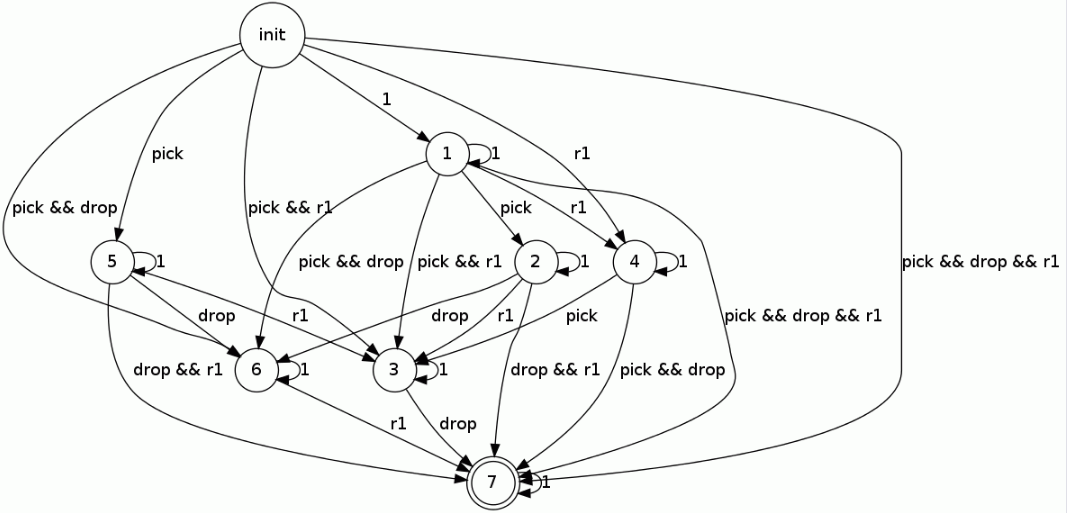
\includegraphics[scale=0.3]{buchiEx1_1}
%\caption{B\"uchi Automaton Corresponding to $\varphi = \diamond (\text{pickrball} \wedge \diamond \text{droprball}) \wedge \diamond %\smallsquare r1$}
%\label{fig:buchiEx1}
%\end{figure*} 

%In the B\"uchi automaton corresponding to this formula as translated by \cite{gastin01}, there are many edges that have \&\& in the label. These paths can only be taken if we satisfy both of the propositions at the same time. However, because in our example the propositions do not overlap (the ball is not in the same room as the basket, and the neither the ball or basket is located in room 1) these edge are impossible to take. Therefore we remove these edges from the automaton. We then have a much simpler automaton that is shown in figure \ref{fig:ex1SimplifiedBuchi}

\begin{figure}
\centering
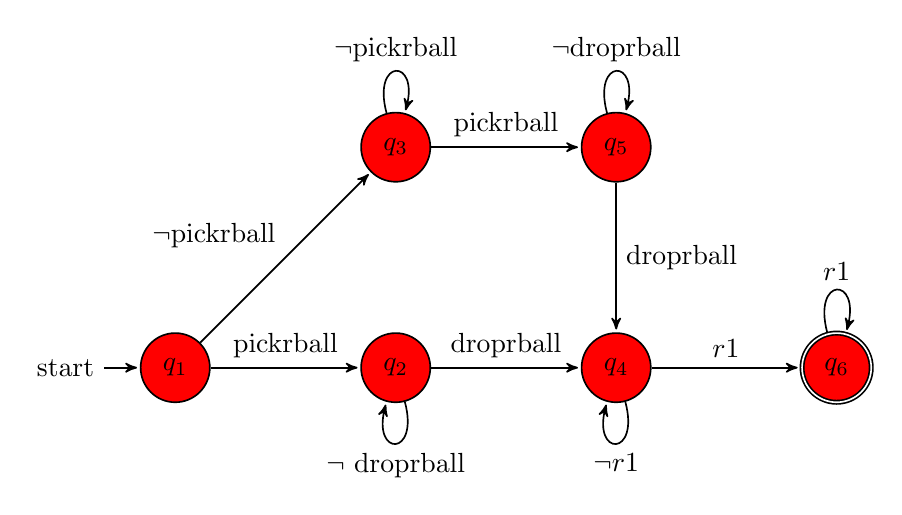
\begin{tikzpicture}[->,>=stealth',shorten >=1pt,auto,node distance=2.8cm,
                    semithick]
  \tikzstyle{every state}=[fill=red,draw=black,text=black]

  \node[initial,state] (A)                    {$q_1$};
  \node[state] (B)                    [right of=A]{$q_2$};
  \node[state] (C)                    [right of=B]{$q_4$};
  \node[state] (E)                    [above of=B]{$q_3$};
  \node[state] (F)                    [above of=C]{$q_5$};
  \node[state,accepting]         (D) [right of=C] {$q_6$};

  \path (A) edge              node {pickrball} (B)
  		%(A) edge [loop above] node {$\neg \pi_1$} (A)
  		(B) edge [loop below] node {$\neg$ droprball} (B)
  		(B) edge              node {droprball} (C)
  		(A) edge              node {$\neg$pickrball} (E)
  		(E) edge              node {pickrball} (F)
  		(F) edge              node {droprball} (C)
  		(C) edge [loop below] node {$\neg r1$} (C)
  		(C) edge              node {$r1$} (D)
  		(E) edge [loop above] node {$\neg$pickrball} (E)
  		(F) edge [loop above] node {$\neg$droprball} (F)
  		(D) edge [loop above] node {$r1$} (D);
\end{tikzpicture}
\caption{Simplified B\"uchi Automaton for $\varphi = \diamond (\text{pickrball} \wedge \diamond \text{droprball}) \wedge \diamond \smallsquare r1$ 1}
\label{fig:ex1SimplifiedBuchi}
\end{figure} 

In this automaton, we can see that $d(q_1)=3$, $d(q_2)=2$, $d(q_3)=3$, $d(q_4)=1$, $d(q_5)=2$, $d(q_6)=0$. For the first time, we have a node connected to the initial node which is on the same level as the initial node. With the greedy algorithm, we see that we will not start a new Dijkstra search until we find a node which is a level bellow our current level. Therefore we will not start a new search until we find a node in the product automaton with projection onto $q_2$ or $q_5$. 

We can also see that from the illustration of the workspace, that the ball (rball) is not located next to the initial node, so the first proposition must be $\neg$pickrball. Examining the automaton in figure \ref{fig:ex1SimplifiedBuchi} we see we are guaranteed to take a path through nodes with projection $q_3$ and that we can never go to a node with the projection $q_2$. Therefore we are in the same situation as for sequencing i.e.\ there is only one sequence of actions that will satisfy the formula, implying that the greedy algorithm will find the same path as the accepted algorithm, just faster. 

\begin{figure}[!htb]
\centering
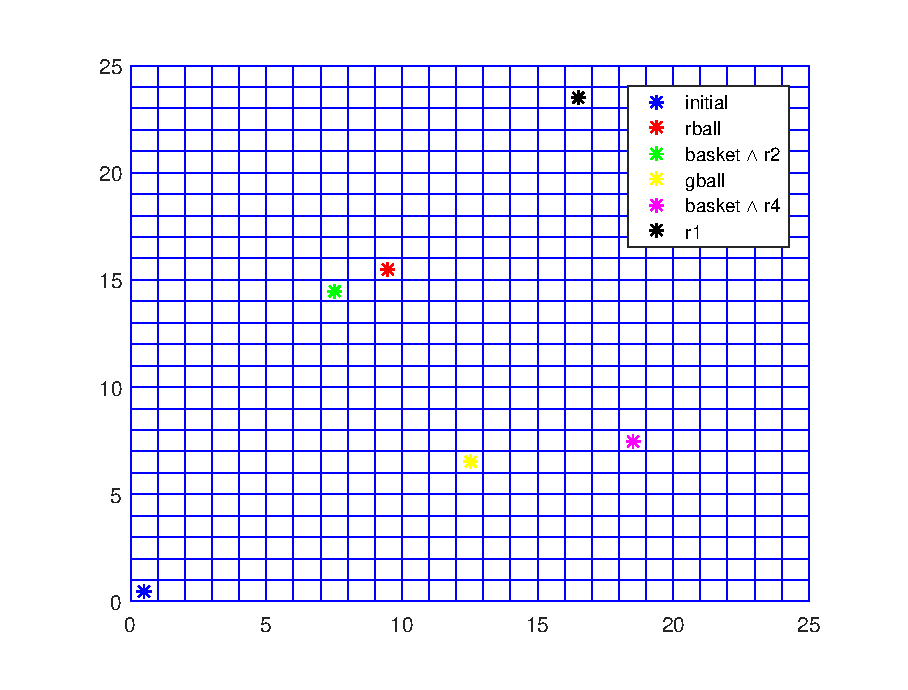
\includegraphics[scale=1]{workspace2.eps}
\label{fig:workspace2}
\caption{Workspace 2}
\end{figure}

We see that this is true in the output of the algorithms. Both give the same sequence of states and actions

%Have to recalculate this!!!!!!
The accepted algorithm gives \\


\begin{minipage}{\textwidth}
\begingroup
\fontsize{9pt}{12pt}\selectfont
\begin{lstlisting}
Accepted Algorithm
==================
accepted_plan done within 0.05s: precost 66.00, sufcost 0.00
\end{lstlisting}
\endgroup
\end{minipage} \\ \\


while the greedy algorithm gives \\


\begin{minipage}{\textwidth}
\begingroup
\fontsize{9pt}{12pt}\selectfont
\begin{lstlisting}
Greedy Algorithm
==================
greedy_plan done within 0.03s: precost 66.00, sufcost 0.00
\end{lstlisting}
\endgroup
\end{minipage} \\ \\


\section{Example 1 Overlapping Regions}
We now look at the same example, except now we have a different workspace. We choose this example to show what happens if the regions of interest are overlapping. Because of the way the code is structured, we are not able to make take transitions with two or more propositions at one time. We show the example if rball is in the same area as the basket. If this is the case, then pickrball and dropbasket could theoretically be done simultaneously. However, this is not possible because of the code. The only possible transitions that we can take that include \&\& have to be a region and a potential task. We leave the transitions satisfying this requirement and remove all others so the algorithm can have a better distances to follow. The automaton is now
\begin{figure}
\centering
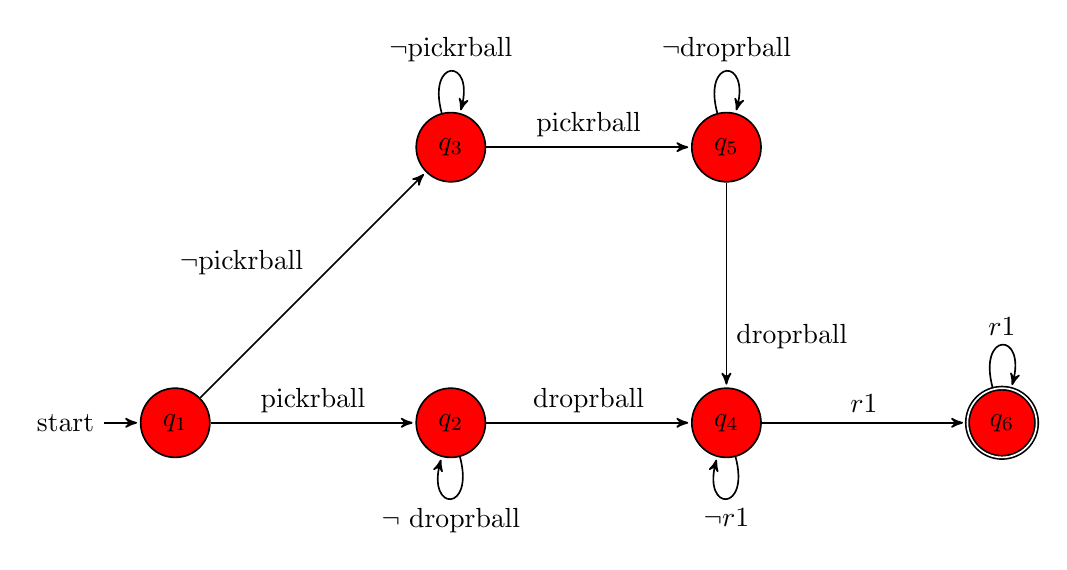
\begin{tikzpicture}[->,>=stealth',shorten >=1pt,auto,node distance=3.5cm,
                    semithick]
  \tikzstyle{every state}=[fill=red,draw=black,text=black]

  \node[initial,state] (A)                    {$q_1$};
  \node[state] (B)                    [right of=A]{$q_2$};
  \node[state] (C)                    [right of=B]{$q_4$};
  \node[state] (E)                    [above of=B]{$q_3$};
  \node[state] (F)                    [above of=C]{$q_5$};
  \node[state,accepting]         (D) [right of=C] {$q_6$};

  \path (A) edge              node {pickrball} (B)
  		%(A) edge   [bend right=90]	 node {rball \&\& basket} (C)
  		%(E) edge		[near start]			node {rball \&\& basket} (C)
  		%(A) edge [loop above] node {$\neg \pi_1$} (A)
  		(B) edge [loop below] node {$\neg$ droprball} (B)
  		(B) edge              node {droprball} (C)
  		(A) edge              node {$\neg$pickrball} (E)
  		(E) edge              node {pickrball} (F)
  		(F) edge        [near end]      node {droprball} (C)
  		(C) edge [loop below] node {$\neg r1$} (C)
  		(C) edge              node {$r1$} (D)
  		(E) edge [loop above] node {$\neg$pickrball} (E)
  		(F) edge [loop above] node {$\neg$droprball} (F)
  		(D) edge [loop above] node {$r1$} (D);
\end{tikzpicture}
\caption{Simplified B\"uchi Automaton Corresponding to $\varphi = \diamond (\text{pickrball} \wedge \diamond \text{droprball}) \wedge \diamond \smallsquare r1$ 2}
\label{fig:ex1OverlapSimplifiedBuchi}
\end{figure} 

In this automaton, we now have $d(q_1)=3$, $d(q_2)=2$, $d(q_3)=3$, $d(q_4)=1$, $d(q_5) = 2$ and $d(q_6)=0$. We see again that rball and basket are not one step away from the initial node, implying that we cannot take the first step pickrball. This means that we can never go to $q_2$, and that there is only one path through the automaton to take. Therefore the greedy algorithm is guaranteed to compute the same path as the accepted algorithm and it will do so in less time.

We look at the results and see that the greedy algorithm indeed calculates the same path in a shorter amount of time than the accepted algorithm. \\


\begin{minipage}{\textwidth}
\begingroup
\fontsize{9pt}{12pt}\selectfont
\begin{lstlisting}
Accepted Algorithm
==================
accepted_plan done within 0.05s: precost 60.00, sufcost 0.00
...
full construction and synthesis done within 1.11s 
\end{lstlisting}
\endgroup
\end{minipage} \\ \\



\begin{minipage}{\textwidth}
\begingroup
\fontsize{9pt}{12pt}\selectfont
\begin{lstlisting}
==================
greedy_plan done within 0.02s: precost 60.00, sufcost 0.00

full construction and synthesis done within 1.09s 
\end{lstlisting}
\endgroup
\end{minipage} \\ \\


\section{Example 2}
We now look at the example taken from \cite{guo15} in which the robot has to pick up and deliver two different balls (rball and gball) to two different baskets, and the robot cannot carry two balls at once. After this is done the robot is to go to r1 and stay there. This task is formalized as 
\begin{align*}
\varphi = \diamond (\text{pickrball} \wedge \diamond (\text{droprball})) \wedge \diamond(\text{pickgball} \wedge \diamond (\text{dropgball})) \wedge \smallsquare (\text{pickrball} \rightarrow \\
 \textbf{X}(\neg \text{pickgball} \U \text{droprball})) \wedge \smallsquare (\text{pickgball} \rightarrow \textbf{X} (\neg \text{pickrball} \U \text{dropgball})) \&\& \diamond \smallsquare r1
\end{align*}
This formula formalizes the basket corresponding to rball is in region r2 and the basket corresponding to gball is in r4. The B\"uchi automaton corresponding to this formula is much to large to show. It has 75 states and 797 edges. If the reader is interested, the automaton can be found using the online tool \cite{ltlbuchiwebsite} with the input F(pickrball \&\& F(droprball)) \&\& F(pickgball \&\& F(dropgball)) \&\& G(pickrball -> X(! pickgball U droprball)) \&\& G(pickgball -> X(! pickrball U dropgball)) \&\& F(G(r1)). It is too large for the tool to give a visual representation but it will provide a list of states and edges.  

To analyse the performance of the greedy algorithm on this problem, we are going to break up this problem into the choices that the robot has. The robot has to pick up one of the balls, return it to the corresponding basket, then pick up the second ball and return it to its corresponding basket. Assuming that everything else is done in the optimal way, the only choice that must be made is which ball to pick up first. This is the output, accepted algorithm first: \\


\begin{minipage}{\textwidth}
\begingroup
\fontsize{9pt}{12pt}\selectfont
\begin{lstlisting}
Accepted Algorithm
==================
accepted_plan done within 0.63s: precost 118.00, sufcost 0.00
...
full construction and synthesis done within 55.25s 
\end{lstlisting}
\endgroup
\end{minipage} \\ \\


and the greedy algorithm \\


\begin{minipage}{\textwidth}
\begingroup
\fontsize{9pt}{12pt}\selectfont
\begin{lstlisting}
==================
greedy_plan done within 0.28s: precost 130.00, sufcost 0.00
...
full construction and synthesis done within 57.55s 
\end{lstlisting}
\endgroup
\end{minipage} \\ \\


as we can see, the greedy algorithm picks the closest ball (rball) first even though it is not optimal overall. The added cost is relatively small though, only 12. However, it is possible that the difference could be much larger. In an analysis of speed, the greedy algorithm does the search faster, In about half the time. In either case, the actual search takes around or less than a hundredth of the total time.

\section{Example 2 Modified}
We now look at a modified version of example two. Say the robot has to pick up and deliver two different balls (rball and gball) to two different baskets, and the robot cannot carry two balls at once and that is it. There is no need to go to r1, or do anything after the balls are returned to their respective baskets. This task is formalized as 
\begin{align*}
\varphi = &\diamond (\text{pickrball} \wedge \diamond (\text{droprball})) \wedge \diamond(\text{pickgball} \wedge \diamond (\text{dropgball})) \wedge \smallsquare (\text{pickrball} \rightarrow \\ 
& \textbf{X}(\neg \text{pickgball} \U \text{droprball})) \wedge \smallsquare (\text{pickgball} \rightarrow \textbf{X} (\neg \text{pickrball} \U \text{dropgball}))
\end{align*}
This version seems easier than original example. The B\"uchi automaton for this formula would seem to agree; it is smaller, with 38 nodes and 308 edges. However, here is the out put from both algorithms: \\


\begin{minipage}{\textwidth}
\begingroup
\fontsize{9pt}{12pt}\selectfont
\begin{lstlisting}
Accepted Algorithm
==================
accepted_plan done within 926.40s: precost 101.00, sufcost 0.00
...
full construction and synthesis done within 950.95s 
\end{lstlisting}
\endgroup
\end{minipage} \\ \\


and from the greedy algorithm \\


\begin{minipage}{\textwidth}
\begingroup
\fontsize{9pt}{12pt}\selectfont
\begin{lstlisting}
Greedy Algorithm
==================
greedy_plan done within 0.30s: precost 104.00, sufcost 0.00
...
full construction and synthesis done within 21.60s
\end{lstlisting} 
\endgroup
\end{minipage} \\ \\


This is by far the largest difference in computation times that we have seen thus far! We will show how this difference is caused by the searches from accepting nodes back to themselves.

As before, we have $|\text{product automaton}| =|\text{FTS}| \times |\text{B\"uchi}| \times |\text{possible actions}|$. The FTS still has 625 nodes, this buchi automaton has 38 nodes, and there are 5 possible actions ("none", "pickrball", "droprball", "pickgball", "dropgball"). This makes for a product automaton of 118750. There are 4 accepting states in the B\"uchi automaton. This gives us 12500 accepting nodes in the product automaton. The accepted algorithm calculates a path back from each accepting node back to itself. This calculation is relatively quick if the accepting node can transition back to itself; however, the cost is much longer if it doesn't. It turns out in this example only 629 of the accepting nodes have a self loop, while 11871 do not. It may seem like the accepting nodes should all be able to transfer back to themselves, but they cannot because of the accepting nodes in the B\"uchi automaton. 

Each accepting node in the B\"uchi automaton has a self loop however, the labels of the self loop can make many of these transitions impossible. The four self loop labels for the four accepting nodes of the B\"uchi automaton are (droprball \&\& dropgball), (!pickrball \&\& dropgball), (!pickrball \&\& !pickgball), and (droprball \&\& !pickgball). Thus the only possible self loop is (!pickrball \&\& !pickgball). All other accepting states must look for another path back to themselves, which results in the incredible increase in time. This is likely the largest danger and downside of using the accepted algorithm. The number of accepting states grows with the size of the FTS, the B\"uchi automaton, and the number of possible actions. Then we have to do a search for each of these accepting nodes.  



\section{Other Examples}
As we have seen, due to the complexity of the B\"uchi automata it can be very hard to analyse the performance of the greedy algorithm compared to the accepted algorithm with respect to cost for more complex formulas. We therefore provide the results of runs for various formulas in table \ref{table}. We use formulas from the table in \cite{somenzi00} to try to show a comprehensive experimentation. The formulas are run on the workspace in figure \ref{fig:workspace2}. 

\begin{landscape}
\begin{table}[]
\centering
\small
\begin{tabular}{|c|c|c|c|c|}
\hline
Formula & \makecell{Accepted Cost \\ prefix, suffix} & Accepted Time & \makecell{Our Cost \\ prefix, suffix} & Our Time \\ \hline
     '(!r223 U r445) || (!r268 U r435)'  &         27, 0     &      0.04         &      27, 0   &     0.01     \\ \hline
      '!r62 U(!r266 U r422)'  &         38, 0     &       0.05        &     38, 0     &     0.02     \\ \hline
       '[]<> r0 -> []<> r317' &         1, 0      &       5.06        &    1, 0      &    0.00     \\ \hline
       '[]<> r0 <-> []<> r317'  & 1, 0		&		10.70		& 1, 0 	&  0.00 \\ \hline 
      '!(<><> r498 <-> r541)' &	42, 0	&	0.03	&	42, 0	&	0.02	\\		\hline
      '!([]<> r3 -> []<>r591)' &	 3, 0	&	5.06 	&	3, 0 	&	0.00	\\		\hline
      '!([]<> r3 <-> []<>r591)' &	 3, 0	&	10.31	&	39, 0	&	0.01	\\		\hline
      '!r532 R (!r432 || r321)' &	 0, 0	&	4.97 	&	0, 0	&	0.01 	\\		\hline
     \makecell{ '<> r114 \&\& [](r114 -> <> r12) \&\& \\((X r114 U X r12) || !X( r114 U r12))' }&	24	&	0.08 	&	24	&	0.01	\\		\hline
   \makecell{ '<> pickrball \&\& [](pickrball -> <> droprball) \\ \&\& ((X pickrball U X droprball) || !X( pickrball U droprball))' } &	47, 0	&	28.87	&	47, 0	&	0.03	\\		\hline
      ' <> r124 \&\& <> !r124' &	28, 0	&	0.05 	&	28, 0	&	0.01	\\		\hline
%      &		&		&		&		\\		\hline
 %     &		&		&		&		\\		\hline
  %    &		&		&		&		\\		\hline
\end{tabular}
\caption{Comparison of Accepted Algorithm with Greedy Algorithm on Various Examples}
\label{table}
\end{table}
\end{landscape}

As we can see, our algorithm always produces a path in a shorter time than the accepted algorithm. However, it can happen that our algorithm produces a plan that is much worse than the accepted algorithm e.g.\ '!([]<> r3 <-> []<>r591)'. 

%\subsection{OR Operator}
%As we have seen in the LTL semantics, LTL formulas can contain an OR Boolean connective i.e.\ $\varphi = \varphi_1 \lor \varphi_2$. In all the other examples that we have seen, the formulas specify tasks and the algorithm has to \textit{at most} choose the order of the tasks. The OR connective introduces the idea that the algorithm has to choose \textit{which} tasks to do. Let us first look at the formula $(\diamond \pi_0 \wedge \diamond \pi_1 ) \lor \diamond \pi_2$.
%The B\"uchi automaton corresponding to this formula as calculated by \cite{gastin01} is shown in figure \ref{fig:ORbuchi}.
%
%\begin{figure}
%\centering
%\begin{tikzpicture}[->,>=stealth',shorten >=1pt,auto,node distance=4cm,
%                    semithick]
%  \tikzstyle{every state}=[fill=red,draw=black,text=black]
%
%  \node[initial,state] (A)                    {$q_1$};
%  \node[state] (B)                    [right of=A]{$q_2$};
%  \node[state] (C)                    [right of=B]{$q_4$};
%  \node[state] (E)                    [below of=C]{$q_3$};
%  \node[state] (F)                    [above of=C]{$q_5$};
%  \node[state,accepting]         (D) [right of=C] {$q_6$};
%
%  \path (A) edge              node {$\neg (\pi_0 \lor \pi_1 \lor  \pi_2)$} (B)
%  		(B) edge   				 node {$\pi_0$} (C)
%  		(B) edge					node {$\pi_1$} (E)
%  		(A) edge					 node {$\neg \pi_2$} (F)
%  		(C) edge 					node {$\pi_1$} (D)
%  		(B) edge              node {$\pi_0$} (C)
%  		(E) edge              node {$\pi_0$} (D)
%  		(F) edge              node {$\pi_2$} (D)
%  		(A) edge              [bend left] node [near end] {$\pi_0$} (C)
%  		(A) edge             node {$\pi_1$} (E)
%  		(A) edge              [bend left] node {$\pi_2$} (D);
%  		%(E) edge [loop above] node {$\neg$rball} (E)
%  		%(F) edge [loop above] node {$\neg$basket} (F)
%  		%(D) edge [loop above] node {$r1$} (D);
%\end{tikzpicture}
%\caption{Simplified B\"uchi Automaton Corresponding to $(\diamond \pi_0 \wedge \diamond \pi_1 ) \lor \diamond \pi_2$}
%\label{fig:ORbuchi}
%\end{figure} 
%
%The distances corresponding to this automaton are $d(q_1) = 1$, $d(q_2) = 2$, $d(q_3)=1$, $d(d_4)=1$, $d(q_5)=1$ and $d(q_6)=0$. As one can see, starting with a distance of 1, the only lower level is 0, which is the accepting level. Therefore our algorithm will only do one Dijkstra search, which is the same as the accepted algorithm. Our algorithm therefore gives the optimal result. 

%\begin{figure}
%\centering
%\begin{tikzpicture}[->,>=stealth',shorten >=1pt,auto,node distance=3.5cm,
%                    semithick]
%  \tikzstyle{every state}=[fill=red,draw=black,text=black]
%
%  \node[initial,state] (A)                    {$q_1$};
%  \node[state] (B)                    [right of=A]{$q_2$};
%  \node[state] (C)                    [below of=B]{$q_3$};
%  \node[state] (D)                    [right of=B]{$q_4$};
%  \node[state] (E)                    [above of=D]{$q_5$};
%  \node[state] (F)                    [right of=C]{$q_6$};
%  \node[state] (G)                    [below of=F]{$q_7$};
%  \node[state,accepting]         (H) [right of=D] {$q_8$};
%
%  \path (A) edge              node {$\neg (\pi_0 \lor \pi_1 \lor  \pi_2 \lor \pi_3)$} (B)
%  		(A) edge   				 node {$\neg (\pi_0 \lor \pi_1 \lor  \pi_2 \lor \pi_3)$} (C)
%  		(A) edge					node {$\pi_0$} (E)
%  		(A) edge			[bend left] node {$\pi_1$} (D)
%  		(A) edge 					node {$\pi_2$} (F)
%  		(A) edge             [bend right] node {$\pi_3$} (G);
%%  		(E) edge              node {$\pi_0$} (D)
%%  		(F) edge              node {$\pi_2$} (D)
%%  		(A) edge              [bend left] node {$\pi_0$} (C)
%%  		(A) edge             node {$\pi_1$} (E)
%%  		(A) edge              [bend left] node {$\pi_2$} (D);
%  		%(E) edge [loop above] node {$\neg$rball} (E)
%  		%(F) edge [loop above] node {$\neg$basket} (F)
%  		%(D) edge [loop above] node {$r1$} (D);
%\end{tikzpicture}
%\caption{Simplified B\"uchi Automaton Corresponding to $(\diamond \pi_0 \wedge \diamond \pi_1 ) \lor (\diamond \pi_2 \wedge \diamond \pi_3)$}
%\label{fig:ORbuchi}
%\end{figure} 

\newpage
\FloatBarrier
\chapter{Appendix}
\begingroup
\fontsize{9pt}{12pt}\selectfont

\begin{lstlisting}[language=Python]
from collections import deque
from heapq import heappush, heappop
from itertools import count
import networkx as nx
from networkx.utils import generate_unique_node
import warnings as _warnings
from networkx import dijkstra_predecessor_and_distance

def adapted_dijkstra_multisource(G, source, cutoff=None, target=None):
    """Uses Dijkstra's algorithm to find shortest weighted paths
    Parameters
    ----------
    G : NetworkX graph
    sources : non-empty iterable of nodes
        Starting nodes for paths. If this is just an iterable containing
        a single node, then all paths computed by this function will
        start from that node. If there are two or more nodes in this
        iterable, the computed paths may begin from any one of the start
        nodes.
    target : node label, optional
        Ending node for path. Search is halted when target is found.
    cutoff : integer or float, optional
        Depth to stop the search. Only return paths with length <= cutoff.
    Returns
    -------
    dist : dictionary
        A mapping from node to shortest distance to that node from one
        of the source nodes.
    next_node : tuple
        The first node, n, the search finds that is one level below the current node
        i.e. d_p(n) = lev - 1
    paths: dictionary
        dict to store the path list from source to each node, keyed by node.
    Notes
    -----
    The optional predecessor and path dictionaries can be accessed by
    the caller through the original pred and paths objects passed
    as arguments. No need to explicitly return pred or paths.
    """

    paths = {source: [source]}

    # define weight function
    weight = lambda u, v, data: data.get('weight', 1)

    # succ = successors
    G_succ = G.succ if G.is_directed() else G.adj

    # rename functions
    push = heappush
    pop = heappop

    dist = {}  # dictionary of final distances
    seen = {}
    # fringe is heapq with 3-tuples (distance,c,node)
    # use the count c to avoid comparing nodes (may not be able to)
    c = count()
    fringe = []
    next_node = []
    # current level of starting node
    cur_level = G.node[source]['dist']
    if cur_level == 0:
        cur_level = 1
    #for source in sources:
    seen[source] = 0
    push(fringe, (0, next(c), source))
    while fringe:
        (d, _, v) = pop(fringe)
        if v in dist:
            continue  # already searched this node.
        dist[v] = d
        if G.node[v]['dist'] < cur_level:
            if cur_level == 1:
                if v in G.predecessors(v):
                    print 'self loop'
                    next_node = v
                    break
                loop_pre, loop_dist = dijkstra_predecessor_and_distance(G, v)
                if v in loop_dist.keys():

                    if loop_dist[v] != 0:
                        print 'not self loop'
                        next_node = v
                        break 
            else:
                next_node = v
                break

        for u, e in G_succ[v].items():
            cost = weight(v, u, e)
            if cost is None:
                continue
            vu_dist = dist[v] + cost
            if cutoff is not None:
                if vu_dist > cutoff:
                    continue
            if u in dist:
                if vu_dist < dist[u]:
                    raise ValueError('Contradictory paths found:',
                                     'negative weights?')
            elif u not in seen or vu_dist < seen[u]:
                seen[u] = vu_dist
                push(fringe, (vu_dist, next(c), u))
                if paths is not None:
                    paths[u] = paths[v] + [u]
    
    return dist, next_node, paths
\end{lstlisting}


\begin{lstlisting} [language=Python]
def greedy_plan(product, beta=10):
	# requires a full construct of product automaton
	# used for 'stadic' and 'ready'
	start = time.time()
	runs = {}
	loop = {}
	cycle = {}
	line = {}
	# 
	# 
	# Find the shortest path
	# to each accepting state
	#
	for prod_init in product.graph['initial']:
		# Find prefix
		lev = product.node[prod_init]['dist']
		start_node = prod_init
		precost = 0
		prefix = [start_node]
		if lev == 0:
			lev = 1
		while lev > 0:

			di,targ,path = ga.adapted_dijkstra_multisource(product,start_node)

			if targ == []:
				print '=================='        
				print 'No accepting run found in planning!'
				return None, None

			lev = product.node[targ]['dist']
			
			start_node = targ

			print start_node
			precost = precost+di[targ]
			if lev == 0:				
				prefix.extend(path[targ][1:])

			else:
				prefix.extend(path[targ][1:-1])

	prod_target = targ

	

	if prod_target in product.predecessors(prod_target):

		loop[prod_target] = (product.edge[prod_target][prod_target]["weight"], [prod_target, prod_target])

		
   	else:

		loop_pre, loop_dist = dijkstra_predecessor_and_distance(product, prod_target)

		for target_pred in product.predecessors_iter(prod_target):

			if target_pred in loop_dist:
				cycle[target_pred] = product.edge[target_pred][prod_target]["weight"] + loop_dist[target_pred]
				
		if cycle:
			opti_pred = min(cycle, key = cycle.get)
			suffix = compute_path_from_pre(loop_pre, opti_pred)
			loop[prod_target] = (cycle[opti_pred], suffix)


	for target in loop.iterkeys():
		if target == targ:
			line[target] = precost+beta*loop[target][0]
		if line:
			runs[(prod_init, targ)] = (prefix, precost, loop[targ][1], loop[targ][0])

	if runs:
		prefix, precost, suffix, sufcost = min(runs.values(), key = lambda p: p[1] + beta*p[3])
		run = ProdAut_Run(product, prefix, precost, suffix, sufcost, precost+beta*sufcost)
		print '=================='
		print 'new_algorithm_plan done within %.2fs: precost %.2f, sufcost %.2f' %(time.time()-start, round(precost), round(sufcost))
		return run, time.time()-start

	print '=================='        
	print 'No accepting run found in optimal planning!'
        return None, None
\end{lstlisting}






%\subsubsection*{Reachability while Avoiding Regions Path}
%\begin{lstlisting}
%------------------------------
%the prefix of plan **states**:
%[((0, 0, 1), 'None'), ((1, 0, 1), 'None'), ((2, 0, 1), 'None'), ((3, 0, 1), 'None'), ((3, 1, 1), 'None'), ((4, 1, 1), 'None'), ((4, 2, 1), 'None'), ((5, 2, 1), 'None'), ((6, 2, 1), 'None'), ((6, 3, 1), 'None'), ((6, 4, 1), 'None'), ((7, 4, 1), 'None'), ((7, 5, 1), 'None'), ((8, 5, 1), 'None'), ((9, 5, 1), 'None'), ((9, 6, 1), 'None'), ((9, 7, 1), 'None'), ((9, 8, 1), 'None'), ((10, 8, 1), 'None'), ((10, 9, 1), 'None'), ((10, 10, 1), 'None'), ((11, 10, 1), 'None'), ((12, 10, 1), 'None'), ((13, 10, 1), 'None'), ((14, 10, 1), 'None'), ((14, 11, 1), 'None'), ((15, 11, 1), 'None'), ((16, 11, 1), 'None'), ((17, 11, 1), 'None'), ((18, 11, 1), 'None'), ((19, 11, 1), 'None'), ((19, 12, 1), 'None'), ((20, 12, 1), 'None'), ((20, 13, 1), 'None'), ((20, 14, 1), 'None'), ((20, 15, 1), 'None'), ((20, 16, 1), 'None')]
%the suffix of plan **states**:
%[((20, 17, 1), 'None'), ((20, 17, 1), 'None')]
%------------------------------
%the prefix of plan **actions**:
%[(0, 0, 1), (1, 0, 1), (2, 0, 1), (3, 0, 1), (3, 1, 1), (4, 1, 1), (4, 2, 1), (5, 2, 1), (6, 2, 1), (6, 3, 1), (6, 4, 1), (7, 4, 1), (7, 5, 1), (8, 5, 1), (9, 5, 1), (9, 6, 1), (9, 7, 1), (9, 8, 1), (10, 8, 1), (10, 9, 1), (10, 10, 1), (11, 10, 1), (12, 10, 1), (13, 10, 1), (14, 10, 1), (14, 11, 1), (15, 11, 1), (16, 11, 1), (17, 11, 1), (18, 11, 1), (19, 11, 1), (19, 12, 1), (20, 12, 1), (20, 13, 1), (20, 14, 1), (20, 15, 1), (20, 16, 1), (20, 17, 1)]
%the suffix of plan **actions**:
%['None', 'None']
%\end{lstlisting}

\subsubsection*{Sequencing Path}
\begin{lstlisting}
------------------------------
the prefix of plan **states**:
[((0, 0, 1), 'None'), ((1, 0, 1), 'None'), ((1, 1, 1), 'None'), ((1, 2, 1), 'None'), ((2, 2, 1), 'None'), ((3, 2, 1), 'None'), ((3, 3, 1), 'None'), ((4, 3, 1), 'None'), ((5, 3, 1), 'None'), ((5, 4, 1), 'None'), ((5, 5, 1), 'None'), ((5, 6, 1), 'None'), ((6, 6, 1), 'None'), ((7, 6, 1), 'None'), ((7, 7, 1), 'None'), ((8, 7, 1), 'None'), ((9, 7, 1), 'None'), ((9, 8, 1), 'None'), ((9, 9, 1), 'None'), ((9, 10, 1), 'None'), ((10, 10, 1), 'None'), ((11, 10, 1), 'None'), ((11, 11, 1), 'None'), ((11, 12, 1), 'None'), ((12, 12, 1), 'None'), ((12, 13, 1), 'None'), ((12, 14, 1), 'None'), ((12, 15, 1), 'None'), ((13, 15, 1), 'None'), ((14, 15, 1), 'None'), ((15, 15, 1), 'None'), ((16, 15, 1), 'None'), ((17, 15, 1), 'None'), ((18, 15, 1), 'None'), ((19, 15, 1), 'None'), ((20, 15, 1), 'None'), ((19, 15, 1), 'None'), ((19, 16, 1), 'None'), ((18, 16, 1), 'None'), ((18, 17, 1), 'None'), ((17, 17, 1), 'None'), ((17, 18, 1), 'None'), ((16, 18, 1), 'None'), ((15, 18, 1), 'None'), ((15, 19, 1), 'None'), ((14, 19, 1), 'None'), ((14, 20, 1), 'None'), ((14, 21, 1), 'None'), ((13, 21, 1), 'None'), ((13, 22, 1), 'None'), ((12, 22, 1), 'None'), ((11, 22, 1), 'None'), ((11, 23, 1), 'None'), ((11, 24, 1), 'None'), ((10, 24, 1), 'None'), ((9, 24, 1), 'None'), ((8, 24, 1), 'None'), ((7, 24, 1), 'None'), ((6, 24, 1), 'None'), ((5, 24, 1), 'None'), ((4, 24, 1), 'None'), ((3, 24, 1), 'None'), ((2, 24, 1), 'None'), ((2, 24, 1), 'None')]
the suffix of plan **states**:
[((2, 24, 1), 'None'), ((2, 24, 1), 'None')]
------------------------------
the prefix of plan **actions**:
[(0, 0, 1), (1, 0, 1), (1, 1, 1), (1, 2, 1), (2, 2, 1), (3, 2, 1), (3, 3, 1), (4, 3, 1), (5, 3, 1), (5, 4, 1), (5, 5, 1), (5, 6, 1), (6, 6, 1), (7, 6, 1), (7, 7, 1), (8, 7, 1), (9, 7, 1), (9, 8, 1), (9, 9, 1), (9, 10, 1), (10, 10, 1), (11, 10, 1), (11, 11, 1), (11, 12, 1), (12, 12, 1), (12, 13, 1), (12, 14, 1), (12, 15, 1), (13, 15, 1), (14, 15, 1), (15, 15, 1), (16, 15, 1), (17, 15, 1), (18, 15, 1), (19, 15, 1), (20, 15, 1), (19, 15, 1), (19, 16, 1), (18, 16, 1), (18, 17, 1), (17, 17, 1), (17, 18, 1), (16, 18, 1), (15, 18, 1), (15, 19, 1), (14, 19, 1), (14, 20, 1), (14, 21, 1), (13, 21, 1), (13, 22, 1), (12, 22, 1), (11, 22, 1), (11, 23, 1), (11, 24, 1), (10, 24, 1), (9, 24, 1), (8, 24, 1), (7, 24, 1), (6, 24, 1), (5, 24, 1), (4, 24, 1), (3, 24, 1), (2, 24, 1), 'None', 'None']
the suffix of plan **actions**:
['None', 'None']
\end{lstlisting}



\subsubsection*{Coverage Path Accepted Algorithm}
\begin{lstlisting}
Accepted Algorithm
==================
Dijkstra_plan_networkX done within 0.08s: precost 59.00, sufcost 0.00
------------------------------
the prefix of plan **states**:
[((0, 0, 1), 'None'), ((1, 0, 1), 'None'), ((2, 0, 1), 'None'), ((2, 1, 1), 'None'), ((2, 2, 1), 'None'), ((2, 3, 1), 'None'), ((2, 4, 1), 'None'), ((2, 5, 1), 'None'), ((2, 6, 1), 'None'), ((2, 7, 1), 'None'), ((2, 8, 1), 'None'), ((2, 9, 1), 'None'), ((2, 10, 1), 'None'), ((2, 11, 1), 'None'), ((2, 12, 1), 'None'), ((2, 13, 1), 'None'), ((2, 14, 1), 'None'), ((2, 15, 1), 'None'), ((2, 16, 1), 'None'), ((2, 17, 1), 'None'), ((2, 18, 1), 'None'), ((2, 19, 1), 'None'), ((2, 20, 1), 'None'), ((2, 21, 1), 'None'), ((2, 22, 1), 'None'), ((2, 23, 1), 'None'), ((2, 24, 1), 'None'), ((2, 23, 1), 'None'), ((2, 22, 1), 'None'), ((2, 21, 1), 'None'), ((3, 21, 1), 'None'), ((4, 21, 1), 'None'), ((5, 21, 1), 'None'), ((5, 20, 1), 'None'), ((5, 19, 1), 'None'), ((6, 19, 1), 'None'), ((7, 19, 1), 'None'), ((8, 19, 1), 'None'), ((9, 19, 1), 'None'), ((9, 18, 1), 'None'), ((10, 18, 1), 'None'), ((11, 18, 1), 'None'), ((12, 18, 1), 'None'), ((12, 17, 1), 'None'), ((12, 16, 1), 'None'), ((12, 15, 1), 'None'), ((12, 14, 1), 'None'), ((12, 13, 1), 'None'), ((12, 12, 1), 'None'), ((13, 12, 1), 'None'), ((14, 12, 1), 'None'), ((14, 13, 1), 'None'), ((15, 13, 1), 'None'), ((16, 13, 1), 'None'), ((16, 14, 1), 'None'), ((17, 14, 1), 'None'), ((18, 14, 1), 'None'), ((18, 15, 1), 'None'), ((19, 15, 1), 'None'), ((20, 15, 1), 'None'), ((20, 15, 1), 'None')]
the suffix of plan **states**:
[((20, 15, 1), 'None'), ((20, 15, 1), 'None')]
------------------------------
the prefix of plan **actions**:
[(0, 0, 1), (1, 0, 1), (2, 0, 1), (2, 1, 1), (2, 2, 1), (2, 3, 1), (2, 4, 1), (2, 5, 1), (2, 6, 1), (2, 7, 1), (2, 8, 1), (2, 9, 1), (2, 10, 1), (2, 11, 1), (2, 12, 1), (2, 13, 1), (2, 14, 1), (2, 15, 1), (2, 16, 1), (2, 17, 1), (2, 18, 1), (2, 19, 1), (2, 20, 1), (2, 21, 1), (2, 22, 1), (2, 23, 1), (2, 24, 1), (2, 23, 1), (2, 22, 1), (2, 21, 1), (3, 21, 1), (4, 21, 1), (5, 21, 1), (5, 20, 1), (5, 19, 1), (6, 19, 1), (7, 19, 1), (8, 19, 1), (9, 19, 1), (9, 18, 1), (10, 18, 1), (11, 18, 1), (12, 18, 1), (12, 17, 1), (12, 16, 1), (12, 15, 1), (12, 14, 1), (12, 13, 1), (12, 12, 1), (13, 12, 1), (14, 12, 1), (14, 13, 1), (15, 13, 1), (16, 13, 1), (16, 14, 1), (17, 14, 1), (18, 14, 1), (18, 15, 1), (19, 15, 1), (20, 15, 1), 'None', 'None']
the suffix of plan **actions**:
['None', 'None']
full construction and synthesis done within 0.43s 
\end{lstlisting}

\subsubsection*{Coverage Path Our Algorithm}
\begin{lstlisting}
Our Algorithm
==================
new_algorithm_plan done within 0.02s: precost 62.00, sufcost 0.00
------------------------------
the prefix of plan **states**:
[((0, 0, 1), 'None'), ((1, 0, 1), 'None'), ((2, 0, 1), 'None'), ((3, 0, 1), 'None'), ((3, 1, 1), 'None'), ((4, 1, 1), 'None'), ((5, 1, 1), 'None'), ((6, 1, 1), 'None'), ((6, 2, 1), 'None'), ((6, 3, 1), 'None'), ((6, 4, 1), 'None'), ((6, 5, 1), 'None'), ((7, 5, 1), 'None'), ((8, 5, 1), 'None'), ((8, 6, 1), 'None'), ((9, 6, 1), 'None'), ((10, 6, 1), 'None'), ((10, 7, 1), 'None'), ((10, 8, 1), 'None'), ((10, 9, 1), 'None'), ((11, 9, 1), 'None'), ((12, 9, 1), 'None'), ((12, 10, 1), 'None'), ((12, 11, 1), 'None'), ((12, 12, 1), 'None'), ((12, 13, 1), 'None'), ((13, 13, 1), 'None'), ((13, 14, 1), 'None'), ((14, 14, 1), 'None'), ((15, 14, 1), 'None'), ((16, 14, 1), 'None'), ((17, 14, 1), 'None'), ((17, 15, 1), 'None'), ((18, 15, 1), 'None'), ((19, 15, 1), 'None'), ((20, 15, 1), 'None'), ((20, 16, 1), 'None'), ((19, 16, 1), 'None'), ((19, 17, 1), 'None'), ((18, 17, 1), 'None'), ((18, 18, 1), 'None'), ((17, 18, 1), 'None'), ((17, 19, 1), 'None'), ((17, 20, 1), 'None'), ((16, 20, 1), 'None'), ((15, 20, 1), 'None'), ((15, 21, 1), 'None'), ((14, 21, 1), 'None'), ((14, 22, 1), 'None'), ((13, 22, 1), 'None'), ((13, 23, 1), 'None'), ((13, 24, 1), 'None'), ((12, 24, 1), 'None'), ((11, 24, 1), 'None'), ((10, 24, 1), 'None'), ((9, 24, 1), 'None'), ((8, 24, 1), 'None'), ((7, 24, 1), 'None'), ((6, 24, 1), 'None'), ((5, 24, 1), 'None'), ((4, 24, 1), 'None'), ((3, 24, 1), 'None')]
the suffix of plan **states**:
[((2, 24, 1), 'None'), ((2, 24, 1), 'None')]
------------------------------
the prefix of plan **actions**:
[(0, 0, 1), (1, 0, 1), (2, 0, 1), (3, 0, 1), (3, 1, 1), (4, 1, 1), (5, 1, 1), (6, 1, 1), (6, 2, 1), (6, 3, 1), (6, 4, 1), (6, 5, 1), (7, 5, 1), (8, 5, 1), (8, 6, 1), (9, 6, 1), (10, 6, 1), (10, 7, 1), (10, 8, 1), (10, 9, 1), (11, 9, 1), (12, 9, 1), (12, 10, 1), (12, 11, 1), (12, 12, 1), (12, 13, 1), (13, 13, 1), (13, 14, 1), (14, 14, 1), (15, 14, 1), (16, 14, 1), (17, 14, 1), (17, 15, 1), (18, 15, 1), (19, 15, 1), (20, 15, 1), (20, 16, 1), (19, 16, 1), (19, 17, 1), (18, 17, 1), (18, 18, 1), (17, 18, 1), (17, 19, 1), (17, 20, 1), (16, 20, 1), (15, 20, 1), (15, 21, 1), (14, 21, 1), (14, 22, 1), (13, 22, 1), (13, 23, 1), (13, 24, 1), (12, 24, 1), (11, 24, 1), (10, 24, 1), (9, 24, 1), (8, 24, 1), (7, 24, 1), (6, 24, 1), (5, 24, 1), (4, 24, 1), (3, 24, 1), (2, 24, 1)]
the suffix of plan **actions**:
['None', 'None']
full construction and synthesis done within 0.38s 
\end{lstlisting}


\subsubsection*{Recurrence (Liveliness) Path}
\begin{lstlisting}
the prefix of plan **states**:
[((0, 0, 1), 'None'), ((1, 0, 1), 'None'), ((2, 0, 1), 'None'), ((3, 0, 1), 'None'), ((3, 1, 1), 'None'), ((4, 1, 1), 'None'), ((5, 1, 1), 'None'), ((6, 1, 1), 'None'), ((6, 2, 1), 'None'), ((6, 3, 1), 'None'), ((6, 4, 1), 'None'), ((6, 5, 1), 'None'), ((7, 5, 1), 'None'), ((8, 5, 1), 'None'), ((8, 6, 1), 'None'), ((9, 6, 1), 'None'), ((10, 6, 1), 'None'), ((10, 7, 1), 'None'), ((10, 8, 1), 'None'), ((10, 9, 1), 'None'), ((11, 9, 1), 'None'), ((12, 9, 1), 'None'), ((12, 10, 1), 'None'), ((12, 11, 1), 'None'), ((12, 12, 1), 'None'), ((12, 13, 1), 'None'), ((12, 14, 1), 'None'), ((13, 14, 1), 'None'), ((13, 15, 1), 'None'), ((14, 15, 1), 'None'), ((15, 15, 1), 'None'), ((16, 15, 1), 'None'), ((17, 15, 1), 'None'), ((18, 15, 1), 'None'), ((19, 15, 1), 'None'), ((20, 15, 1), 'None'), ((19, 15, 1), 'None'), ((19, 16, 1), 'None'), ((18, 16, 1), 'None'), ((18, 17, 1), 'None'), ((17, 17, 1), 'None'), ((16, 17, 1), 'None'), ((16, 18, 1), 'None'), ((15, 18, 1), 'None'), ((15, 19, 1), 'None'), ((14, 19, 1), 'None'), ((14, 20, 1), 'None'), ((14, 21, 1), 'None'), ((13, 21, 1), 'None'), ((13, 22, 1), 'None'), ((12, 22, 1), 'None'), ((11, 22, 1), 'None'), ((11, 23, 1), 'None'), ((11, 24, 1), 'None'), ((10, 24, 1), 'None'), ((9, 24, 1), 'None'), ((8, 24, 1), 'None'), ((7, 24, 1), 'None'), ((6, 24, 1), 'None'), ((5, 24, 1), 'None'), ((4, 24, 1), 'None'), ((3, 24, 1), 'None')]
the suffix of plan **states**:
[((2, 24, 1), 'None'), ((2, 23, 1), 'None'), ((2, 22, 1), 'None'), ((2, 21, 1), 'None'), ((3, 21, 1), 'None'), ((3, 20, 1), 'None'), ((4, 20, 1), 'None'), ((5, 20, 1), 'None'), ((6, 20, 1), 'None'), ((6, 19, 1), 'None'), ((6, 18, 1), 'None'), ((6, 17, 1), 'None'), ((7, 17, 1), 'None'), ((7, 16, 1), 'None'), ((8, 16, 1), 'None'), ((9, 16, 1), 'None'), ((10, 16, 1), 'None'), ((10, 15, 1), 'None'), ((10, 14, 1), 'None'), ((10, 13, 1), 'None'), ((11, 13, 1), 'None'), ((11, 12, 1), 'None'), ((12, 12, 1), 'None'), ((12, 13, 1), 'None'), ((12, 14, 1), 'None'), ((13, 14, 1), 'None'), ((13, 15, 1), 'None'), ((14, 15, 1), 'None'), ((15, 15, 1), 'None'), ((16, 15, 1), 'None'), ((17, 15, 1), 'None'), ((18, 15, 1), 'None'), ((19, 15, 1), 'None'), ((20, 15, 1), 'None'), ((19, 15, 1), 'None'), ((19, 16, 1), 'None'), ((18, 16, 1), 'None'), ((18, 17, 1), 'None'), ((17, 17, 1), 'None'), ((16, 17, 1), 'None'), ((16, 18, 1), 'None'), ((15, 18, 1), 'None'), ((15, 19, 1), 'None'), ((14, 19, 1), 'None'), ((14, 20, 1), 'None'), ((14, 21, 1), 'None'), ((13, 21, 1), 'None'), ((13, 22, 1), 'None'), ((12, 22, 1), 'None'), ((11, 22, 1), 'None'), ((11, 23, 1), 'None'), ((11, 24, 1), 'None'), ((10, 24, 1), 'None'), ((9, 24, 1), 'None'), ((8, 24, 1), 'None'), ((7, 24, 1), 'None'), ((6, 24, 1), 'None'), ((5, 24, 1), 'None'), ((4, 24, 1), 'None'), ((3, 24, 1), 'None'), ((2, 24, 1), 'None')]
------------------------------
the prefix of plan **actions**:
[(0, 0, 1), (1, 0, 1), (2, 0, 1), (3, 0, 1), (3, 1, 1), (4, 1, 1), (5, 1, 1), (6, 1, 1), (6, 2, 1), (6, 3, 1), (6, 4, 1), (6, 5, 1), (7, 5, 1), (8, 5, 1), (8, 6, 1), (9, 6, 1), (10, 6, 1), (10, 7, 1), (10, 8, 1), (10, 9, 1), (11, 9, 1), (12, 9, 1), (12, 10, 1), (12, 11, 1), (12, 12, 1), (12, 13, 1), (12, 14, 1), (13, 14, 1), (13, 15, 1), (14, 15, 1), (15, 15, 1), (16, 15, 1), (17, 15, 1), (18, 15, 1), (19, 15, 1), (20, 15, 1), (19, 15, 1), (19, 16, 1), (18, 16, 1), (18, 17, 1), (17, 17, 1), (16, 17, 1), (16, 18, 1), (15, 18, 1), (15, 19, 1), (14, 19, 1), (14, 20, 1), (14, 21, 1), (13, 21, 1), (13, 22, 1), (12, 22, 1), (11, 22, 1), (11, 23, 1), (11, 24, 1), (10, 24, 1), (9, 24, 1), (8, 24, 1), (7, 24, 1), (6, 24, 1), (5, 24, 1), (4, 24, 1), (3, 24, 1), (2, 24, 1)]
the suffix of plan **actions**:
[(2, 23, 1), (2, 22, 1), (2, 21, 1), (3, 21, 1), (3, 20, 1), (4, 20, 1), (5, 20, 1), (6, 20, 1), (6, 19, 1), (6, 18, 1), (6, 17, 1), (7, 17, 1), (7, 16, 1), (8, 16, 1), (9, 16, 1), (10, 16, 1), (10, 15, 1), (10, 14, 1), (10, 13, 1), (11, 13, 1), (11, 12, 1), (12, 12, 1), (12, 13, 1), (12, 14, 1), (13, 14, 1), (13, 15, 1), (14, 15, 1), (15, 15, 1), (16, 15, 1), (17, 15, 1), (18, 15, 1), (19, 15, 1), (20, 15, 1), (19, 15, 1), (19, 16, 1), (18, 16, 1), (18, 17, 1), (17, 17, 1), (16, 17, 1), (16, 18, 1), (15, 18, 1), (15, 19, 1), (14, 19, 1), (14, 20, 1), (14, 21, 1), (13, 21, 1), (13, 22, 1), (12, 22, 1), (11, 22, 1), (11, 23, 1), (11, 24, 1), (10, 24, 1), (9, 24, 1), (8, 24, 1), (7, 24, 1), (6, 24, 1), (5, 24, 1), (4, 24, 1), (3, 24, 1), (2, 24, 1), 'None']
\end{lstlisting} 


\subsubsection*{Example 1}
\begin{lstlisting}
------------------------------
the prefix of plan **states**:
[((0, 0, 1), 'None'), ((0, 1, 1), 'None'), ((0, 2, 1), 'None'), ((1, 2, 1), 'None'), ((1, 3, 1), 'None'), ((2, 3, 1), 'None'), ((2, 4, 1), 'None'), ((3, 4, 1), 'None'), ((4, 4, 1), 'None'), ((4, 5, 1), 'None'), ((5, 5, 1), 'None'), ((5, 6, 1), 'None'), ((5, 7, 1), 'None'), ((6, 7, 1), 'None'), ((6, 8, 1), 'None'), ((7, 8, 1), 'None'), ((8, 8, 1), 'None'), ((8, 9, 1), 'None'), ((9, 9, 1), 'None'), ((9, 10, 1), 'None'), ((9, 11, 1), 'None'), ((9, 12, 1), 'None'), ((9, 13, 1), 'None'), ((9, 14, 1), 'None'), ((9, 15, 1), 'None'), ((9, 15, 1), 'pickrball'), ((9, 14, 1), 'None'), ((8, 14, 1), 'None'), ((7, 14, 1), 'None'), ((7, 14, 1), 'droprball'), ((7, 15, 1), 'None'), ((7, 16, 1), 'None'), ((7, 17, 1), 'None'), ((8, 17, 1), 'None'), ((9, 17, 1), 'None'), ((10, 17, 1), 'None'), ((11, 17, 1), 'None'), ((12, 17, 1), 'None'), ((13, 17, 1), 'None'), ((14, 17, 1), 'None'), ((15, 17, 1), 'None'), ((16, 17, 1), 'None'), ((17, 17, 1), 'None'), ((18, 17, 1), 'None'), ((19, 17, 1), 'None'), ((20, 17, 1), 'None'), ((21, 17, 1), 'None'), ((22, 17, 1), 'None'), ((23, 17, 1), 'None'), ((23, 17, 1), 'None')]
the suffix of plan **states**:
[((23, 17, 1), 'None'), ((23, 17, 1), 'None')]
------------------------------
the prefix of plan **actions**:
[(0, 0, 1), (0, 1, 1), (0, 2, 1), (1, 2, 1), (1, 3, 1), (2, 3, 1), (2, 4, 1), (3, 4, 1), (4, 4, 1), (4, 5, 1), (5, 5, 1), (5, 6, 1), (5, 7, 1), (6, 7, 1), (6, 8, 1), (7, 8, 1), (8, 8, 1), (8, 9, 1), (9, 9, 1), (9, 10, 1), (9, 11, 1), (9, 12, 1), (9, 13, 1), (9, 14, 1), (9, 15, 1), 'pickrball', (9, 14, 1), (8, 14, 1), (7, 14, 1), 'droprball', (7, 15, 1), (7, 16, 1), (7, 17, 1), (8, 17, 1), (9, 17, 1), (10, 17, 1), (11, 17, 1), (12, 17, 1), (13, 17, 1), (14, 17, 1), (15, 17, 1), (16, 17, 1), (17, 17, 1), (18, 17, 1), (19, 17, 1), (20, 17, 1), (21, 17, 1), (22, 17, 1), (23, 17, 1), 'None', 'None']
the suffix of plan **actions**:
['None', 'None']
\end{lstlisting}

\subsubsection*{Example 1 Overlapping}
\begin{lstlisting}
------------------------------
the prefix of plan **states**:
[((0, 0, 1), 'None'), ((0, 1, 1), 'None'), ((0, 2, 1), 'None'), ((1, 2, 1), 'None'), ((1, 3, 1), 'None'), ((2, 3, 1), 'None'), ((2, 4, 1), 'None'), ((3, 4, 1), 'None'), ((4, 4, 1), 'None'), ((4, 5, 1), 'None'), ((5, 5, 1), 'None'), ((5, 6, 1), 'None'), ((5, 7, 1), 'None'), ((6, 7, 1), 'None'), ((6, 8, 1), 'None'), ((7, 8, 1), 'None'), ((8, 8, 1), 'None'), ((8, 9, 1), 'None'), ((9, 9, 1), 'None'), ((9, 10, 1), 'None'), ((9, 11, 1), 'None'), ((9, 12, 1), 'None'), ((9, 13, 1), 'None'), ((9, 14, 1), 'None'), ((9, 15, 1), 'None'), ((9, 15, 1), 'pickrball'), ((9, 15, 1), 'droprball'), ((10, 15, 1), 'None'), ((10, 16, 1), 'None'), ((11, 16, 1), 'None'), ((12, 16, 1), 'None'), ((12, 17, 1), 'None'), ((13, 17, 1), 'None'), ((14, 17, 1), 'None'), ((15, 17, 1), 'None'), ((16, 17, 1), 'None'), ((17, 17, 1), 'None'), ((18, 17, 1), 'None'), ((19, 17, 1), 'None'), ((20, 17, 1), 'None'), ((21, 17, 1), 'None'), ((22, 17, 1), 'None'), ((23, 17, 1), 'None'), ((23, 17, 1), 'None')]
the suffix of plan **states**:
[((23, 17, 1), 'None'), ((23, 17, 1), 'None')]
------------------------------
the prefix of plan **actions**:
[(0, 0, 1), (0, 1, 1), (0, 2, 1), (1, 2, 1), (1, 3, 1), (2, 3, 1), (2, 4, 1), (3, 4, 1), (4, 4, 1), (4, 5, 1), (5, 5, 1), (5, 6, 1), (5, 7, 1), (6, 7, 1), (6, 8, 1), (7, 8, 1), (8, 8, 1), (8, 9, 1), (9, 9, 1), (9, 10, 1), (9, 11, 1), (9, 12, 1), (9, 13, 1), (9, 14, 1), (9, 15, 1), 'pickrball', 'droprball', (10, 15, 1), (10, 16, 1), (11, 16, 1), (12, 16, 1), (12, 17, 1), (13, 17, 1), (14, 17, 1), (15, 17, 1), (16, 17, 1), (17, 17, 1), (18, 17, 1), (19, 17, 1), (20, 17, 1), (21, 17, 1), (22, 17, 1), (23, 17, 1), 'None', 'None']
the suffix of plan **actions**:
['None', 'None']
\end{lstlisting}


\subsubsection{Example 2 Accepted Algorithm Path}
\begin{lstlisting}
------------------------------
the prefix of plan **states**:
[((0, 0, 1), 'None'), ((1, 0, 1), 'None'), ((1, 1, 1), 'None'), ((2, 1, 1), 'None'), ((2, 2, 1), 'None'), ((3, 2, 1), 'None'), ((3, 3, 1), 'None'), ((4, 3, 1), 'None'), ((5, 3, 1), 'None'), ((6, 3, 1), 'None'), ((7, 3, 1), 'None'), ((8, 3, 1), 'None'), ((8, 4, 1), 'None'), ((9, 4, 1), 'None'), ((10, 4, 1), 'None'), ((11, 4, 1), 'None'), ((12, 4, 1), 'None'), ((13, 4, 1), 'None'), ((14, 4, 1), 'None'), ((15, 4, 1), 'None'), ((16, 4, 1), 'None'), ((16, 5, 1), 'None'), ((16, 6, 1), 'None'), ((17, 6, 1), 'None'), ((18, 6, 1), 'None'), ((19, 6, 1), 'None'), ((19, 7, 1), 'None'), ((19, 8, 1), 'None'), ((19, 8, 1), 'pickgball'), ((19, 9, 1), 'None'), ((18, 9, 1), 'None'), ((18, 10, 1), 'None'), ((17, 10, 1), 'None'), ((16, 10, 1), 'None'), ((15, 10, 1), 'None'), ((14, 10, 1), 'None'), ((13, 10, 1), 'None'), ((12, 10, 1), 'None'), ((11, 10, 1), 'None'), ((10, 10, 1), 'None'), ((9, 10, 1), 'None'), ((8, 10, 1), 'None'), ((7, 10, 1), 'None'), ((6, 10, 1), 'None'), ((5, 10, 1), 'None'), ((4, 10, 1), 'None'), ((3, 10, 1), 'None'), ((2, 10, 1), 'None'), ((2, 10, 1), 'dropgball'), ((2, 11, 1), 'None'), ((2, 12, 1), 'None'), ((2, 13, 1), 'None'), ((2, 14, 1), 'None'), ((3, 14, 1), 'None'), ((4, 14, 1), 'None'), ((5, 14, 1), 'None'), ((5, 15, 1), 'None'), ((6, 15, 1), 'None'), ((7, 15, 1), 'None'), ((8, 15, 1), 'None'), ((9, 15, 1), 'None'), ((9, 15, 1), 'pickrball'), ((8, 15, 1), 'None'), ((7, 15, 1), 'None'), ((7, 14, 1), 'None'), ((7, 14, 1), 'droprball'), ((8, 14, 1), 'None'), ((8, 15, 1), 'None'), ((9, 15, 1), 'None'), ((10, 15, 1), 'None'), ((11, 15, 1), 'None'), ((12, 15, 1), 'None'), ((12, 16, 1), 'None'), ((13, 16, 1), 'None'), ((14, 16, 1), 'None'), ((15, 16, 1), 'None'), ((16, 16, 1), 'None'), ((17, 16, 1), 'None'), ((18, 16, 1), 'None'), ((19, 16, 1), 'None'), ((20, 16, 1), 'None'), ((21, 16, 1), 'None'), ((22, 16, 1), 'None'), ((22, 16, 1), 'None')]
the suffix of plan **states**:
[((22, 16, 1), 'None'), ((22, 16, 1), 'None')]
------------------------------
the prefix of plan **actions**:
[(0, 0, 1), (1, 0, 1), (1, 1, 1), (2, 1, 1), (2, 2, 1), (3, 2, 1), (3, 3, 1), (4, 3, 1), (5, 3, 1), (6, 3, 1), (7, 3, 1), (8, 3, 1), (8, 4, 1), (9, 4, 1), (10, 4, 1), (11, 4, 1), (12, 4, 1), (13, 4, 1), (14, 4, 1), (15, 4, 1), (16, 4, 1), (16, 5, 1), (16, 6, 1), (17, 6, 1), (18, 6, 1), (19, 6, 1), (19, 7, 1), (19, 8, 1), 'pickgball', (19, 9, 1), (18, 9, 1), (18, 10, 1), (17, 10, 1), (16, 10, 1), (15, 10, 1), (14, 10, 1), (13, 10, 1), (12, 10, 1), (11, 10, 1), (10, 10, 1), (9, 10, 1), (8, 10, 1), (7, 10, 1), (6, 10, 1), (5, 10, 1), (4, 10, 1), (3, 10, 1), (2, 10, 1), 'dropgball', (2, 11, 1), (2, 12, 1), (2, 13, 1), (2, 14, 1), (3, 14, 1), (4, 14, 1), (5, 14, 1), (5, 15, 1), (6, 15, 1), (7, 15, 1), (8, 15, 1), (9, 15, 1), 'pickrball', (8, 15, 1), (7, 15, 1), (7, 14, 1), 'droprball', (8, 14, 1), (8, 15, 1), (9, 15, 1), (10, 15, 1), (11, 15, 1), (12, 15, 1), (12, 16, 1), (13, 16, 1), (14, 16, 1), (15, 16, 1), (16, 16, 1), (17, 16, 1), (18, 16, 1), (19, 16, 1), (20, 16, 1), (21, 16, 1), (22, 16, 1), 'None', 'None']
the suffix of plan **actions**:
['None', 'None']
\end{lstlisting}

\subsubsection{Example 2 Our Algorithm Path}
%\subsection{Our Algorithm}
\begin{lstlisting}
------------------------------
the prefix of plan **states**:
[((0, 0, 1), 'None'), ((0, 1, 1), 'None'), ((0, 2, 1), 'None'), ((1, 2, 1), 'None'), ((2, 2, 1), 'None'), ((3, 2, 1), 'None'), ((4, 2, 1), 'None'), ((4, 3, 1), 'None'), ((5, 3, 1), 'None'), ((5, 4, 1), 'None'), ((6, 4, 1), 'None'), ((7, 4, 1), 'None'), ((7, 5, 1), 'None'), ((8, 5, 1), 'None'), ((8, 6, 1), 'None'), ((8, 7, 1), 'None'), ((8, 8, 1), 'None'), ((8, 9, 1), 'None'), ((9, 9, 1), 'None'), ((9, 10, 1), 'None'), ((9, 11, 1), 'None'), ((9, 12, 1), 'None'), ((9, 13, 1), 'None'), ((9, 14, 1), 'None'), ((9, 15, 1), 'None'), ((9, 15, 1), 'pickrball'), ((9, 14, 1), 'None'), ((8, 14, 1), 'None'), ((7, 14, 1), 'None'), ((7, 14, 1), 'droprball'), ((8, 14, 1), 'None'), ((8, 13, 1), 'None'), ((8, 12, 1), 'None'), ((9, 12, 1), 'None'), ((10, 12, 1), 'None'), ((11, 12, 1), 'None'), ((11, 11, 1), 'None'), ((11, 10, 1), 'None'), ((12, 10, 1), 'None'), ((12, 9, 1), 'None'), ((13, 9, 1), 'None'), ((14, 9, 1), 'None'), ((15, 9, 1), 'None'), ((15, 8, 1), 'None'), ((16, 8, 1), 'None'), ((17, 8, 1), 'None'), ((18, 8, 1), 'None'), ((19, 8, 1), 'None'), ((19, 8, 1), 'pickgball'), ((18, 8, 1), 'None'), ((18, 9, 1), 'None'), ((18, 10, 1), 'None'), ((17, 10, 1), 'None'), ((16, 10, 1), 'None'), ((15, 10, 1), 'None'), ((14, 10, 1), 'None'), ((13, 10, 1), 'None'), ((12, 10, 1), 'None'), ((11, 10, 1), 'None'), ((10, 10, 1), 'None'), ((9, 10, 1), 'None'), ((8, 10, 1), 'None'), ((7, 10, 1), 'None'), ((6, 10, 1), 'None'), ((5, 10, 1), 'None'), ((4, 10, 1), 'None'), ((3, 10, 1), 'None'), ((2, 10, 1), 'None'), ((2, 10, 1), 'dropgball'), ((2, 11, 1), 'None'), ((2, 12, 1), 'None'), ((2, 13, 1), 'None'), ((3, 13, 1), 'None'), ((3, 14, 1), 'None'), ((4, 14, 1), 'None'), ((4, 15, 1), 'None'), ((4, 16, 1), 'None'), ((5, 16, 1), 'None'), ((6, 16, 1), 'None'), ((7, 16, 1), 'None'), ((8, 16, 1), 'None'), ((9, 16, 1), 'None'), ((10, 16, 1), 'None'), ((11, 16, 1), 'None'), ((12, 16, 1), 'None'), ((13, 16, 1), 'None'), ((14, 16, 1), 'None'), ((15, 16, 1), 'None'), ((16, 16, 1), 'None'), ((17, 16, 1), 'None'), ((18, 16, 1), 'None'), ((19, 16, 1), 'None'), ((20, 16, 1), 'None'), ((21, 16, 1), 'None'), ((22, 16, 1), 'None'), ((22, 16, 1), 'None')]
the suffix of plan **states**:
[((22, 16, 1), 'None'), ((22, 16, 1), 'None')]
------------------------------
the prefix of plan **actions**:
[(0, 0, 1), (0, 1, 1), (0, 2, 1), (1, 2, 1), (2, 2, 1), (3, 2, 1), (4, 2, 1), (4, 3, 1), (5, 3, 1), (5, 4, 1), (6, 4, 1), (7, 4, 1), (7, 5, 1), (8, 5, 1), (8, 6, 1), (8, 7, 1), (8, 8, 1), (8, 9, 1), (9, 9, 1), (9, 10, 1), (9, 11, 1), (9, 12, 1), (9, 13, 1), (9, 14, 1), (9, 15, 1), 'pickrball', (9, 14, 1), (8, 14, 1), (7, 14, 1), 'droprball', (8, 14, 1), (8, 13, 1), (8, 12, 1), (9, 12, 1), (10, 12, 1), (11, 12, 1), (11, 11, 1), (11, 10, 1), (12, 10, 1), (12, 9, 1), (13, 9, 1), (14, 9, 1), (15, 9, 1), (15, 8, 1), (16, 8, 1), (17, 8, 1), (18, 8, 1), (19, 8, 1), 'pickgball', (18, 8, 1), (18, 9, 1), (18, 10, 1), (17, 10, 1), (16, 10, 1), (15, 10, 1), (14, 10, 1), (13, 10, 1), (12, 10, 1), (11, 10, 1), (10, 10, 1), (9, 10, 1), (8, 10, 1), (7, 10, 1), (6, 10, 1), (5, 10, 1), (4, 10, 1), (3, 10, 1), (2, 10, 1), 'dropgball', (2, 11, 1), (2, 12, 1), (2, 13, 1), (3, 13, 1), (3, 14, 1), (4, 14, 1), (4, 15, 1), (4, 16, 1), (5, 16, 1), (6, 16, 1), (7, 16, 1), (8, 16, 1), (9, 16, 1), (10, 16, 1), (11, 16, 1), (12, 16, 1), (13, 16, 1), (14, 16, 1), (15, 16, 1), (16, 16, 1), (17, 16, 1), (18, 16, 1), (19, 16, 1), (20, 16, 1), (21, 16, 1), (22, 16, 1), 'None', 'None']
the suffix of plan **actions**:
['None', 'None']
\end{lstlisting}


\subsubsection{Example 2 Modified Accepted Algorithm Path}
%\subsection{Accepted}
\begin{lstlisting}
------------------------------
the prefix of plan **states**:
[((0, 0, 1), 'None'), ((1, 0, 1), 'None'), ((1, 1, 1), 'None'), ((1, 2, 1), 'None'), ((2, 2, 1), 'None'), ((2, 3, 1), 'None'), ((3, 3, 1), 'None'), ((4, 3, 1), 'None'), ((5, 3, 1), 'None'), ((6, 3, 1), 'None'), ((7, 3, 1), 'None'), ((7, 4, 1), 'None'), ((8, 4, 1), 'None'), ((9, 4, 1), 'None'), ((10, 4, 1), 'None'), ((11, 4, 1), 'None'), ((12, 4, 1), 'None'), ((12, 5, 1), 'None'), ((12, 6, 1), 'None'), ((13, 6, 1), 'None'), ((13, 7, 1), 'None'), ((13, 8, 1), 'None'), ((14, 8, 1), 'None'), ((15, 8, 1), 'None'), ((16, 8, 1), 'None'), ((17, 8, 1), 'None'), ((18, 8, 1), 'None'), ((19, 8, 1), 'None'), ((19, 8, 1), 'pickgball'), ((18, 8, 1), 'None'), ((17, 8, 1), 'None'), ((17, 9, 1), 'None'), ((17, 10, 1), 'None'), ((16, 10, 1), 'None'), ((15, 10, 1), 'None'), ((14, 10, 1), 'None'), ((13, 10, 1), 'None'), ((12, 10, 1), 'None'), ((11, 10, 1), 'None'), ((10, 10, 1), 'None'), ((9, 10, 1), 'None'), ((8, 10, 1), 'None'), ((7, 10, 1), 'None'), ((6, 10, 1), 'None'), ((5, 10, 1), 'None'), ((4, 10, 1), 'None'), ((3, 10, 1), 'None'), ((2, 10, 1), 'None'), ((2, 10, 1), 'dropgball'), ((2, 11, 1), 'None'), ((2, 12, 1), 'None'), ((2, 13, 1), 'None'), ((3, 13, 1), 'None'), ((4, 13, 1), 'None'), ((5, 13, 1), 'None'), ((5, 14, 1), 'None'), ((6, 14, 1), 'None'), ((6, 15, 1), 'None'), ((7, 15, 1), 'None'), ((8, 15, 1), 'None'), ((9, 15, 1), 'None'), ((9, 15, 1), 'pickrball'), ((9, 14, 1), 'None'), ((8, 14, 1), 'None'), ((7, 14, 1), 'None'), ((7, 14, 1), 'droprball'), ((7, 14, 1), 'None')]
the suffix of plan **states**:
[((7, 14, 1), 'None'), ((7, 14, 1), 'None')]
------------------------------
the prefix of plan **actions**:
[(0, 0, 1), (1, 0, 1), (1, 1, 1), (1, 2, 1), (2, 2, 1), (2, 3, 1), (3, 3, 1), (4, 3, 1), (5, 3, 1), (6, 3, 1), (7, 3, 1), (7, 4, 1), (8, 4, 1), (9, 4, 1), (10, 4, 1), (11, 4, 1), (12, 4, 1), (12, 5, 1), (12, 6, 1), (13, 6, 1), (13, 7, 1), (13, 8, 1), (14, 8, 1), (15, 8, 1), (16, 8, 1), (17, 8, 1), (18, 8, 1), (19, 8, 1), 'pickgball', (18, 8, 1), (17, 8, 1), (17, 9, 1), (17, 10, 1), (16, 10, 1), (15, 10, 1), (14, 10, 1), (13, 10, 1), (12, 10, 1), (11, 10, 1), (10, 10, 1), (9, 10, 1), (8, 10, 1), (7, 10, 1), (6, 10, 1), (5, 10, 1), (4, 10, 1), (3, 10, 1), (2, 10, 1), 'dropgball', (2, 11, 1), (2, 12, 1), (2, 13, 1), (3, 13, 1), (4, 13, 1), (5, 13, 1), (5, 14, 1), (6, 14, 1), (6, 15, 1), (7, 15, 1), (8, 15, 1), (9, 15, 1), 'pickrball', (9, 14, 1), (8, 14, 1), (7, 14, 1), 'droprball', 'None', 'None']
the suffix of plan **actions**:
['None', 'None']
\end{lstlisting}

\subsubsection{Example 2 Modified Our Algorithm Path}
\begin{lstlisting}
------------------------------
the prefix of plan **states**:
[((0, 0, 1), 'None'), ((1, 0, 1), 'None'), ((1, 1, 1), 'None'), ((2, 1, 1), 'None'), ((2, 2, 1), 'None'), ((2, 3, 1), 'None'), ((3, 3, 1), 'None'), ((4, 3, 1), 'None'), ((5, 3, 1), 'None'), ((5, 4, 1), 'None'), ((6, 4, 1), 'None'), ((6, 5, 1), 'None'), ((7, 5, 1), 'None'), ((7, 6, 1), 'None'), ((7, 7, 1), 'None'), ((8, 7, 1), 'None'), ((9, 7, 1), 'None'), ((9, 8, 1), 'None'), ((9, 9, 1), 'None'), ((9, 10, 1), 'None'), ((9, 11, 1), 'None'), ((9, 12, 1), 'None'), ((9, 13, 1), 'None'), ((9, 14, 1), 'None'), ((9, 15, 1), 'None'), ((9, 15, 1), 'pickrball'), ((9, 14, 1), 'None'), ((8, 14, 1), 'None'), ((7, 14, 1), 'None'), ((7, 14, 1), 'droprball'), ((7, 13, 1), 'None'), ((8, 13, 1), 'None'), ((8, 12, 1), 'None'), ((8, 11, 1), 'None'), ((9, 11, 1), 'None'), ((9, 10, 1), 'None'), ((9, 9, 1), 'None'), ((9, 8, 1), 'None'), ((10, 8, 1), 'None'), ((11, 8, 1), 'None'), ((12, 8, 1), 'None'), ((13, 8, 1), 'None'), ((14, 8, 1), 'None'), ((15, 8, 1), 'None'), ((16, 8, 1), 'None'), ((17, 8, 1), 'None'), ((18, 8, 1), 'None'), ((19, 8, 1), 'None'), ((19, 8, 1), 'pickgball'), ((18, 8, 1), 'None'), ((17, 8, 1), 'None'), ((17, 9, 1), 'None'), ((16, 9, 1), 'None'), ((16, 10, 1), 'None'), ((15, 10, 1), 'None'), ((14, 10, 1), 'None'), ((13, 10, 1), 'None'), ((12, 10, 1), 'None'), ((11, 10, 1), 'None'), ((10, 10, 1), 'None'), ((9, 10, 1), 'None'), ((8, 10, 1), 'None'), ((7, 10, 1), 'None'), ((6, 10, 1), 'None'), ((5, 10, 1), 'None'), ((4, 10, 1), 'None'), ((3, 10, 1), 'None'), ((2, 10, 1), 'None'), ((2, 10, 1), 'dropgball'), ((2, 10, 1), 'None')]
the suffix of plan **states**:
[((2, 10, 1), 'None'), ((2, 10, 1), 'None')]
------------------------------
the prefix of plan **actions**:
[(0, 0, 1), (1, 0, 1), (1, 1, 1), (2, 1, 1), (2, 2, 1), (2, 3, 1), (3, 3, 1), (4, 3, 1), (5, 3, 1), (5, 4, 1), (6, 4, 1), (6, 5, 1), (7, 5, 1), (7, 6, 1), (7, 7, 1), (8, 7, 1), (9, 7, 1), (9, 8, 1), (9, 9, 1), (9, 10, 1), (9, 11, 1), (9, 12, 1), (9, 13, 1), (9, 14, 1), (9, 15, 1), 'pickrball', (9, 14, 1), (8, 14, 1), (7, 14, 1), 'droprball', (7, 13, 1), (8, 13, 1), (8, 12, 1), (8, 11, 1), (9, 11, 1), (9, 10, 1), (9, 9, 1), (9, 8, 1), (10, 8, 1), (11, 8, 1), (12, 8, 1), (13, 8, 1), (14, 8, 1), (15, 8, 1), (16, 8, 1), (17, 8, 1), (18, 8, 1), (19, 8, 1), 'pickgball', (18, 8, 1), (17, 8, 1), (17, 9, 1), (16, 9, 1), (16, 10, 1), (15, 10, 1), (14, 10, 1), (13, 10, 1), (12, 10, 1), (11, 10, 1), (10, 10, 1), (9, 10, 1), (8, 10, 1), (7, 10, 1), (6, 10, 1), (5, 10, 1), (4, 10, 1), (3, 10, 1), (2, 10, 1), 'dropgball', 'None', 'None']
the suffix of plan **actions**:
['None', 'None']
\end{lstlisting}

\endgroup
%\input{intro}

\newpage
\FloatBarrier
\bibliography{bibliography}
\bibliographystyle{plain}


\end{document}